%% History:
% Pavel Tvrdik (26.12.2004)
%  + initial version for PhD Report
% Daniel Sykora (27.01.2005)
% Michal Valenta (3.12.2008)
% rada zmen ve formatovani (diky M. Duškovi, J. Holubovi a J. Žďárkovi)
% sjednoceni zdrojoveho kodu pro anglickou, ceskou, bakalarskou a diplomovou praci

% One-page layout: (proof-)reading on display
%%%% \documentclass[11pt,oneside,a4paper]{book}
% Two-page layout: final printing
\documentclass[11pt,twoside,a4paper]{book}   
%=-=-=-=-=-=-=-=-=-=-=-=--=%
% The user of this template may find useful to have an alternative to these 
% officially suggested packages:
\usepackage[czech, english]{babel}
\usepackage[T1]{fontenc} % pouzije EC fonty 
% pripadne pisete-li cesky, pak lze zkusit take:
\usepackage[OT1]{fontenc} 
\usepackage[utf8]{inputenc}
\usepackage{lmodern}
%=-=-=-=-=-=-=-=-=-=-=-=--=
%=-=-=-=-=-=-=-=-=-=-=-=--=%
% Depending on your particular TeX distribution and version of conversion tools 
% (dvips/dvipdf/ps2pdf), some (advanced | desperate) users may prefer to use 
% different settings.
% Please uncomment the following style and use your CSLaTeX (cslatex/pdfcslatex) 
% to process your work. Note however, this file is in UTF-8 and a conversion to 
% your native encoding may be required. Some settings below depend on babel 
% macros and should also be modified. See \selectlanguage \iflanguage.
%\usepackage{czech}  %%%%%\usepackage[T1]{czech} %%%%[IL2] [T1] [OT1]
%=-=-=-=-=-=-=-=-=-=-=-=--=%

%%%%%%%%%%%%%%%%%%%%%%%%%%%%%%%%%%%%%%%
% Styles required in your work follow %
%%%%%%%%%%%%%%%%%%%%%%%%%%%%%%%%%%%%%%%
\usepackage{graphicx}
\usepackage{indentfirst} %1. odstavec jako v cestine.

\usepackage{k336_thesis_macros} % specialni makra pro formatovani DP a BP
 % muzete si vytvorit i sva vlastni v souboru k336_thesis_macros.sty
 % najdete  radu jednoduchych definic, ktere zde ani nejsou pouzity
 % napriklad: 
 % \newcommand{\bfig}{\begin{figure}\begin{center}}
 % \newcommand{\efig}{\end{center}\end{figure}}
 % umoznuje pouzit prikaz \bfig namisto \begin{figure}\begin{center} atd.

\newcommand\TypeOfWork{Bakalářská práce}  \typeout{Bakalarska prace}
\newcommand\StudProgram{Softwarové technologie a management, Bakalářský}
\newcommand\StudBranch{Web a multimedia}                  % pro STM

\newcommand\WorkTitle{Planární segmentace mračna bodů}
\newcommand\FirstandFamilyName{Daniel Princ}
\newcommand\Supervisor{Ing. David Sedláček}


% Pouzijete-li pdflatex, tak je prijemne, kdyz bude mit vase prace funkcni odkazy i v pdf formatu
\usepackage[
pdftitle={\WorkTitle},
pdfauthor={\FirstandFamilyName},
bookmarks=true,
colorlinks=true,
breaklinks=true,
urlcolor=red,
citecolor=blue,
linkcolor=blue,
unicode=true,
]
{hyperref}


% Extension posted by Petr Dlouhy in order for better sources reference (\cite{} command) especially in Czech.
% April 2010
% See comment over \thebibliography command for details.
\usepackage[square, numbers]{natbib}             % sazba pouzite literatury
%\usepackage{url}
%\DeclareUrlCommand\url{\def\UrlLeft{<}\def\UrlRight{>}\urlstyle{tt}}  %rm/sf/tt
%\renewcommand{\emph}[1]{\textsl{#1}}    % melo by byt kurziva nebo sklonene,
\let\oldUrl\url
\renewcommand\url[1]{<\texttt{\oldUrl{#1}}>}


\begin{document}
\selectlanguage{czech}
% prikaz \typeout vypise vyse uvedena nastaveni v prikazovem okne
% pro pohodlne ladeni prace
 \typeout{************************************************}
 \typeout{Zvoleny jazyk: cestina}
 \typeout{Typ prace: \TypeOfWork}
 \typeout{Studijni program: \StudProgram}
 \typeout{Obor: \StudBranch}
 \typeout{Jmeno: \FirstandFamilyName}
 \typeout{Nazev prace: \WorkTitle}
 \typeout{Vedouci prace: \Supervisor}
 \typeout{***************************************************}
 \newcommand\Department{Katedra počítačů}
 \newcommand\Faculty{Fakulta elektrotechnická}
 \newcommand\University{České vysoké učení technické v Praze}
 \newcommand\labelSupervisor{Vedoucí práce}
 \newcommand\labelStudProgram{Studijní program}
 \newcommand\labelStudBranch{Obor}


%%%%%%%%%%%%%%%%%%%%%%%%%%    Poznamky ke kompletaci prace
% Nasledujici pasaz uzavrenou v {} ve sve praci samozrejme 
% zakomentujte nebo odstrante. 
% Ve vysledne svazane praci bude nahrazena skutecnym 
% oficialnim zadanim vasi prace.
%{
%\pagenumbering{roman}\setcounter{page}{1}\cleardoublepage \thispagestyle{empty}
%\chapter*{Na tomto místě bude oficiální zadání vaší práce}
%\begin{itemize}
%\item Toto zadání je podepsané děkanem a vedoucím katedry,
%\item musíte si ho vyzvednout na studiijním oddělení Katedry počítačů na Karlově náměstí,
%\item v jedné odevzdané práci bude originál tohoto zadání (originál zůstává po obhajobě na katedře),
%\item ve druhé bude na stejném místě neověřená kopie tohoto dokumentu (tato se vám vrátí po obhajobě).
%\end{itemize}
%\newpage
%}

%%%%%%%%%%%%%%%%%%%%%%%%%%    Titulni stranka / Title page 
\coverpagestarts

%%%%%%%%%%%%%%%%%%%%%%%%%%%    Podekovani / Acknowledgements 
\acknowledgements
\noindent
Zde můžete napsat své poděkování, pokud chcete a máte komu děkovat.


%%%%%%%%%%%%%%%%%%%%%%%%%%%   Prohlaseni / Declaration 
\declaration{V~Praze dne 25.\,5.\,2015}


%%%%%%%%%%%%%%%%%%%%%%%%%%%%    Abstract 
\abstractpage

Translation of Czech abstract into English.

% Prace v cestine musi krome abstraktu v anglictine obsahovat i
% abstrakt v cestine.
\vglue60mm

\noindent{\Huge \textbf{Abstrakt}}
\vskip 2.75\baselineskip

\noindent
Tato bakalářská práce se zabývá problematikou zpracování mračna bodů, konkrétně segmentací na planární
primitiva. Toto má uplatnění zejména při digitální 3D rekonstrukci objektů reálného světa. V současné době je
snaha co nejvíce automatizovat proces zpracování naměřených dat, planární segmentace je jednou ze základních
částí tohoto procesu.

Konkrétním cílem této bakalářské práce je implementovat dva algoritmy, které budou segmentaci provádět co
nejvíce automaticky a zároveň v dostatečné kvalitě. Algoritmy jsou implementovány jako součást 3D
rekonstrukčního nástroje ArchiRec3D.

%%%%%%%%%%%%%%%%%%%%%%%%%%%%%%%%  Obsah / Table of Contents 
\tableofcontents

%%%%%%%%%%%%%%%%%%%%%%%%%%%%%%%  Seznam obrazku / List of Figures 
\listoffigures

%%%%%%%%%%%%%%%%%%%%%%%%%%%%%%%  Seznam tabulek / List of Tables
\listoftables

%**************************************************************

\mainbodystarts
% horizontalní mezera mezi dvema odstavci
%\parskip=5pt
\normalfont
\parskip=0.4\baselineskip plus 0.2\baselineskip minus 0.1\baselineskip

% Odsazeni prvniho radku odstavce resi class book (neaplikuje se na prvni 
% odstavce kapitol, sekci, podsekci atd.) Viz usepackage{indentfirst}.
% Chcete-li selektivne zamezit odsazeni 1. radku nektereho odstavce,
% pouzijte prikaz \noindent.

%**************************************************************

% Pro snadnejsi praci s vetsimi texty je rozumne tyto rozdelit
% do samostatnych souboru nejlepe dle kapitol a tyto potom vkladat
% pomoci prikazu \include{jmeno_souboru.tex} nebo \include{jmeno_souboru}.
% Napr.:
% \include{1_uvod}
% \include{2_teorie}
% atd...
%*****************************************************************************
\chapter{Úvod}
Rekonstrukce 3D modelů se dnes uplatňuje v mnoha oborech. Běžně se můžeme setkat např. s vizualizacemi, které
se často využívají pro simulaci vzhledu města při výstavbě nových objektů. V takovém případě se obvykle
naskenuje aktuální stav okolí výstavby, do kterého se přidá model plánované budovy. Výsledná vizualizace poté
umožňuje posoudit vliv nové výstavby v kontextu okolí. Výhoda je také v tom, že takovéto simulace snadno pochopí i
laický pozorovatel. Využití lze nalézt i v technické praxi, kde mohou 3D modely zachytit aktuální stav
zařízení (např. potrubí v elektrárně), které nemusí odpovídat zastaralé či nekompletní dokumentaci. Přesné 3D
modely krajiny se mohou využívat např. při modelování záplav nebo šíření bezdrátového signálu. Podobně se
modely mohou využívat k modelování šíření zvuku v uzavřených prostorech. Dále můžeme najít rozsáhlé využití v
archeologii a ochraně kulturního dědictví, v dokumentaci důlních děl, monitorování krajiny pro detekci
nebezpečných sesuvů, mapování pobřežních oblastí a mořského dna v okolí přístavů apod.

Existuje několik metod, které se ke sběru těchto dat využívají. Tradiční metodou je fotogrammetrie, kdy se
informace o objektu získávají z několika fotografií a pro případné zpřesnění se může využít geodetického
zaměření. Hlavní nevýhodou této metody je přesnost naměřených dat, která výrazně klesá se vzdáleností měření.
Tato metoda nám obvykle poskytuje souřadnice charakteristických bodů, jako jsou hrany, vrcholy apod. To může
být velká nevýhoda zejména u nepravidelných objektů.

Jednou z nejnovějších metod sběru dat je laserové skenování. Jeho hlavní výhodou je rychlý sběr velkého
množství přesných dat v terénu. Nevýhodou oproti předchozí metodě je zejména špatná identifikace hran a
vrcholů. Další nevýhodou může být fakt, že přístroje pro laserové skenování jsou velmi drahé. Slabinou této
metody je také náročné zpracování, které se neobejde bez výkonné výpočetní techniky. Základním výstupem z
laserového skenování je mračno bodů. Jedná se o tisíce až miliony bodů, které jsou definovány třemi
kartézskými souřadnicemi (x, y, z), dále mohou obsahovat informaci o barvě (r, g, b) a případně také normálu
(n$_x$, n$_y$, n$_z$) k ploše, na které se bod vyskytuje.

\section{Segmentace mračna bodů}

V této práci se zabývám zpracováním mračna bodů, konkrétně jeho planární segmentací. Cílem práce je tedy
identifikovat ve vstupním mračnu bodů rovinné útvary, přiřadit jednotlivé body do těchto rovinných útvarů a
případně zahodit body, které v žádné rovinně neleží (viz Obr. \ref{fig:ukazkova-scena}). Tato segmentace
má smysl zejména v architektuře a archeologii, tedy při rekonstrukci budov a podobných objektů, které jsou
složeny z relativně malého počtu velkých rovin (tedy stěny, střechy apod.).

\begin{figure}[ht]
\begin{center}
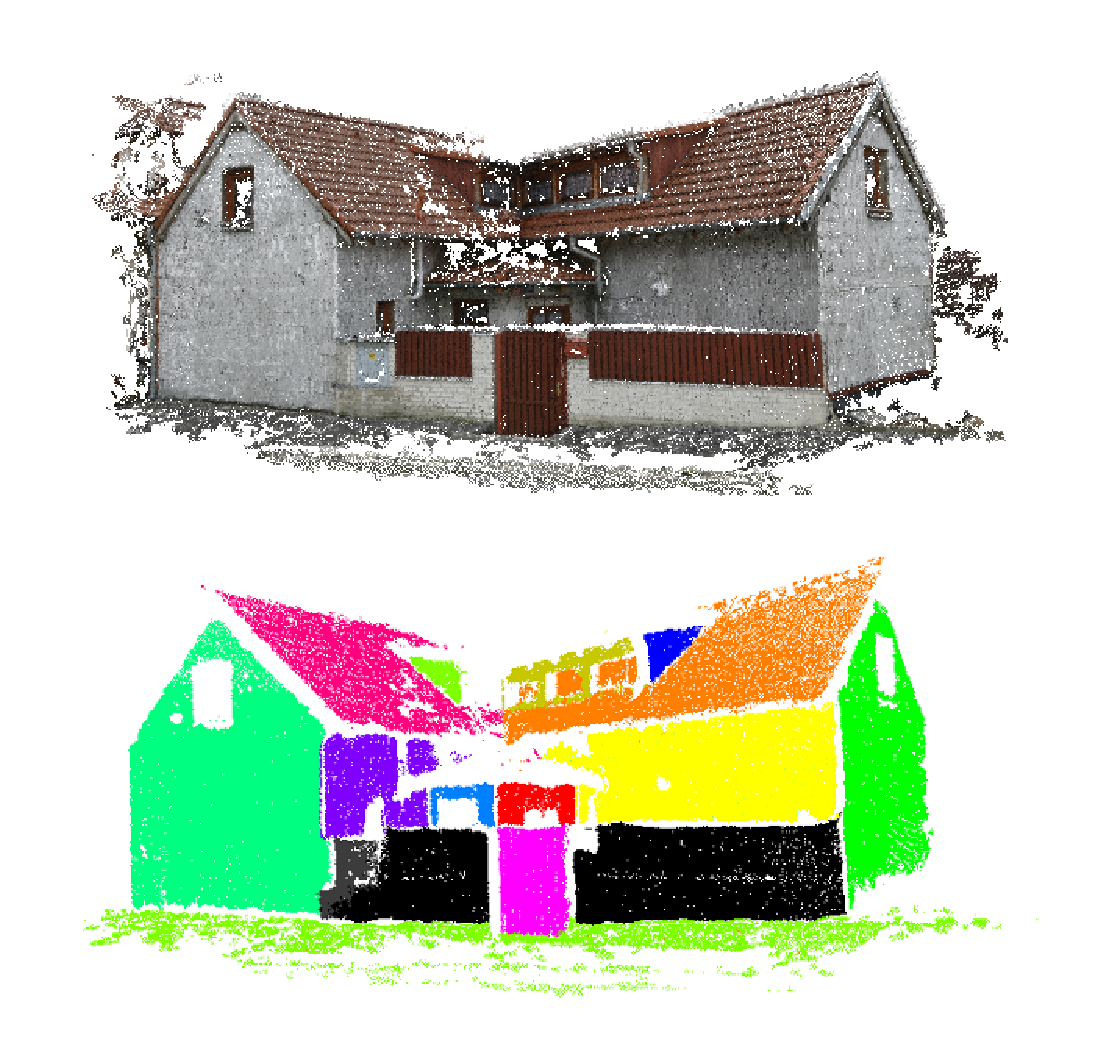
\includegraphics[height=10cm]{figures/1-1-segmentace}
\caption{Ukázková scéna (nahoře) a její planární segmentace (dole).}
\label{fig:ukazkova-scena}
\end{center}
\end{figure}

Segmentační metody můžeme hrubě rozdělit do dvou základních kategorií \cite{Voss04}. Jednak jsou to metody, které segmentují na základě vlastností jako je vzdálenost bodů v prostoru a případně podobnost lokálně odhadnutých normál. Sem spadají např. metody, jako je segmentace na základě skenovacích linií\footnote{V anglické literatuře se označuje jako \uv{scan line segmentation} \cite{Voss04}} nebo surface growing. První zmíněná metoda vychází z toho, že data jsou pořizována postupně podél skenovacích linií. Body v těchto liniích jsou nejprve rozděleny do rovných přímek a poté jsou ve 3D prostoru na základě podobných atributů slučovány do jednotlivých segmentů. Surface growing algoritmy fungují tak, že je vybrán rovinný či nerovinný prvek (seed region) a ten je poté postupně spojován s blízkými body, které mají podobné atributy. Tato metoda je ale silně závislá na volbě vhodného původního prvku.

Do druhé kategorie spadají metody, které přímo odhadují parametry roviny na základě shlukování bodů a vyhledávání lokálních maxim v prostoru parametrů. Sem patří např. rozšíření Houghovi transformace pro 3D prostor. Jeden bod v mračnu, který se nachází na ploše v objektovém prostoru definuje rovinu v prostoru parametrů. Body na stejné ploše mají poté podobné parametry (vzdálenost od počátku a naklonění rovinny) a na základě těchto paramterů jsou poté shlukovány. Jednotlivé shluky bodů pak podle dalších kritérií vytvoří jeden segment. Tato a další podobné metody mají zejména výpočetní problémy, protože mají velké paměťové nároky. Obvyklým problémem obou výše zmíněných kategorií je fakt, že jednotlivé metody se často zaměřují pouze na specifický typ vstupních dat (letecké skeny nebo pozemní skeny).

Článek \cite{Seg01} navrhuje řešení, které zohledňuje jak podobnost bodů v protstoru atributů, tak vzdálenost bodů v objektovém prostoru. Zároveň snižuje počet atributů pro vyšší efektivitu a menší paměťové nároky. Dále by také metoda neměla být závislá na typu vstupních dat.


\section{Struktura práce}

Tato práce nejprve popisuje zadané algoritmy \cite{Seg01} a \cite{Seg02} a věnuje se návrhu obou implementací. Poté následuje část popisující samotnou implementaci algoritmů. Algoritmy jsou implementovány v rámci dodaného nástroje ArchiRec3D \cite{AR3D}, který je psaný v jazyku Java. V závěrečné části práce je otestována správná funkčnost obou algoritmů na uměle generovaných datech a na reálných datech je otestována kvalita algoritmů a jejich implementací. V závěru jsou  shrnuty výsledky testování a analyzovány nedostatky algoritmů. Je zda také zhodnoceno, zda jsou nedostatky způsobeny návrhem algoritmu nebo jeho implementací.


%*****************************************************************************
%\chapter{Popis problému, specifikace cíle}

%\begin{itemize}
%\item Vysvětlení pojmů
%\item Popis řešeného problému, vymezení cílů DP/BP a požadavků na implementovaný systém.
%\item Popis struktury DP/BP ve vztahu k vytyčeným cílům.
%\item Rešeršní zpracování existujících implementací, pokud jsou známy.
%\end{itemize}

%*****************************************************************************
\chapter{Analýza a návrh řešení}

\section{Segmentace na základě velikosti normálového vektoru}

Navržený proces segmentace v článku \cite{Seg01} zahrnuje tři hlavní kroky - definice okolí, výpočet atributů a klastrování bodů. Definice okolí bodu bere v úvahu 3D vzdálenost mezi body a tvar povrchu, na kterém se bod nachází. Atributy daného bodu jsou poté vypočteny na základě tohoto definovaného okolí, pro nižší paměťové nároky jsou pro každý bod použity pouze dva parametry. Po vypočtení parametrů je provedeno klastrování bodů ležících na stejné ploše, které zohledňuje jak podobnost v prostoru atributů, tak vzdálenost bodů v prostoru.

\subsection{Adaptivní válcová definice okolí} 
\label{sub:def-okoli}

Správná definice okolí bodu je zásadní podmínkou pro správnou funkčnost algoritmu, protože okolí bodu přímo ovlivňuje parametry, které jsou pro daný bod vypočteny. V tomto algoritmu je okolí definováno tak, že bere v úvahu vzdálenost bodů v prostoru, ale zároveň také tvar povrchu, na kterém se bod nachází. To znamená, že do okolí jsou zahrnuty pouze takové body, které jsou prostorově blízko, ale zároveň leží na stejné ploše.

Proces definice okolí je znázorněn v diagramu na obrázku \ref{fig:diagram-okoli}. Prvním krokem je vytvořit kouli se středem v bodu, pro který okolí definujeme. Poloměr koule volíme takový, aby koule obsahovala dostatečný počet bodů pro spolehlivý výpočet parametrů. Tuto hodnotu nejde přesněji specifikovat, musí být odvozena z konkrétního mračna bodů, které zpracováváme\footnote{Nicméně praxe ukazuje, že vhodná volba jsou řádově desítky až stovky bodů uvnitř koule.}. Body, které leží uvnitř této koule, proložíme pomocí metody nejmenších čtverců výchozí rovinnou (viz Obr. \ref{fig:definice-okoli}). Poté, co je rovina proložena, vypočítáme pro každý bod v kouli jeho vzdálenost od této roviny. Inverzi této vzdálenosti použijeme v další iteraci jako váhu bodu\footnote{Jednoduše řečeno, čím je bod od plochy dál, tím je jeho váha nižší.}, jak můžeme vidět v rovnici \ref{eq:vypocet-vahy}:
\begin{equation}
p_i = 1/d_i
\label{eq:vypocet-vahy}
\end{equation}
kde $p_i$ značí váhu i-tého bodu a  $d_i$ je vzdálenost bodu od proložené roviny. Tento proces \uv{převažování roviny} se iterativně opakuje, dokud se roviny v rámci iterací již nemění nebo dokud není dosaženo daného počtu iterací (např. 10). Poté je rovnoběžně nad a pod výslednou rovinou definován buffer. Velikost tohoto bufferu je závislá na očekávané velikosti šumu ve vstupních datech. Body, které jsou uvnitř tohoto bufferu, tvoří výsledné okolí (viz Obr. \ref{fig:definice-okoli}(b)). Ostatní body mimo buffer se již na okolí nijak nepodílejí.

\begin{figure}[ht]
\begin{center}
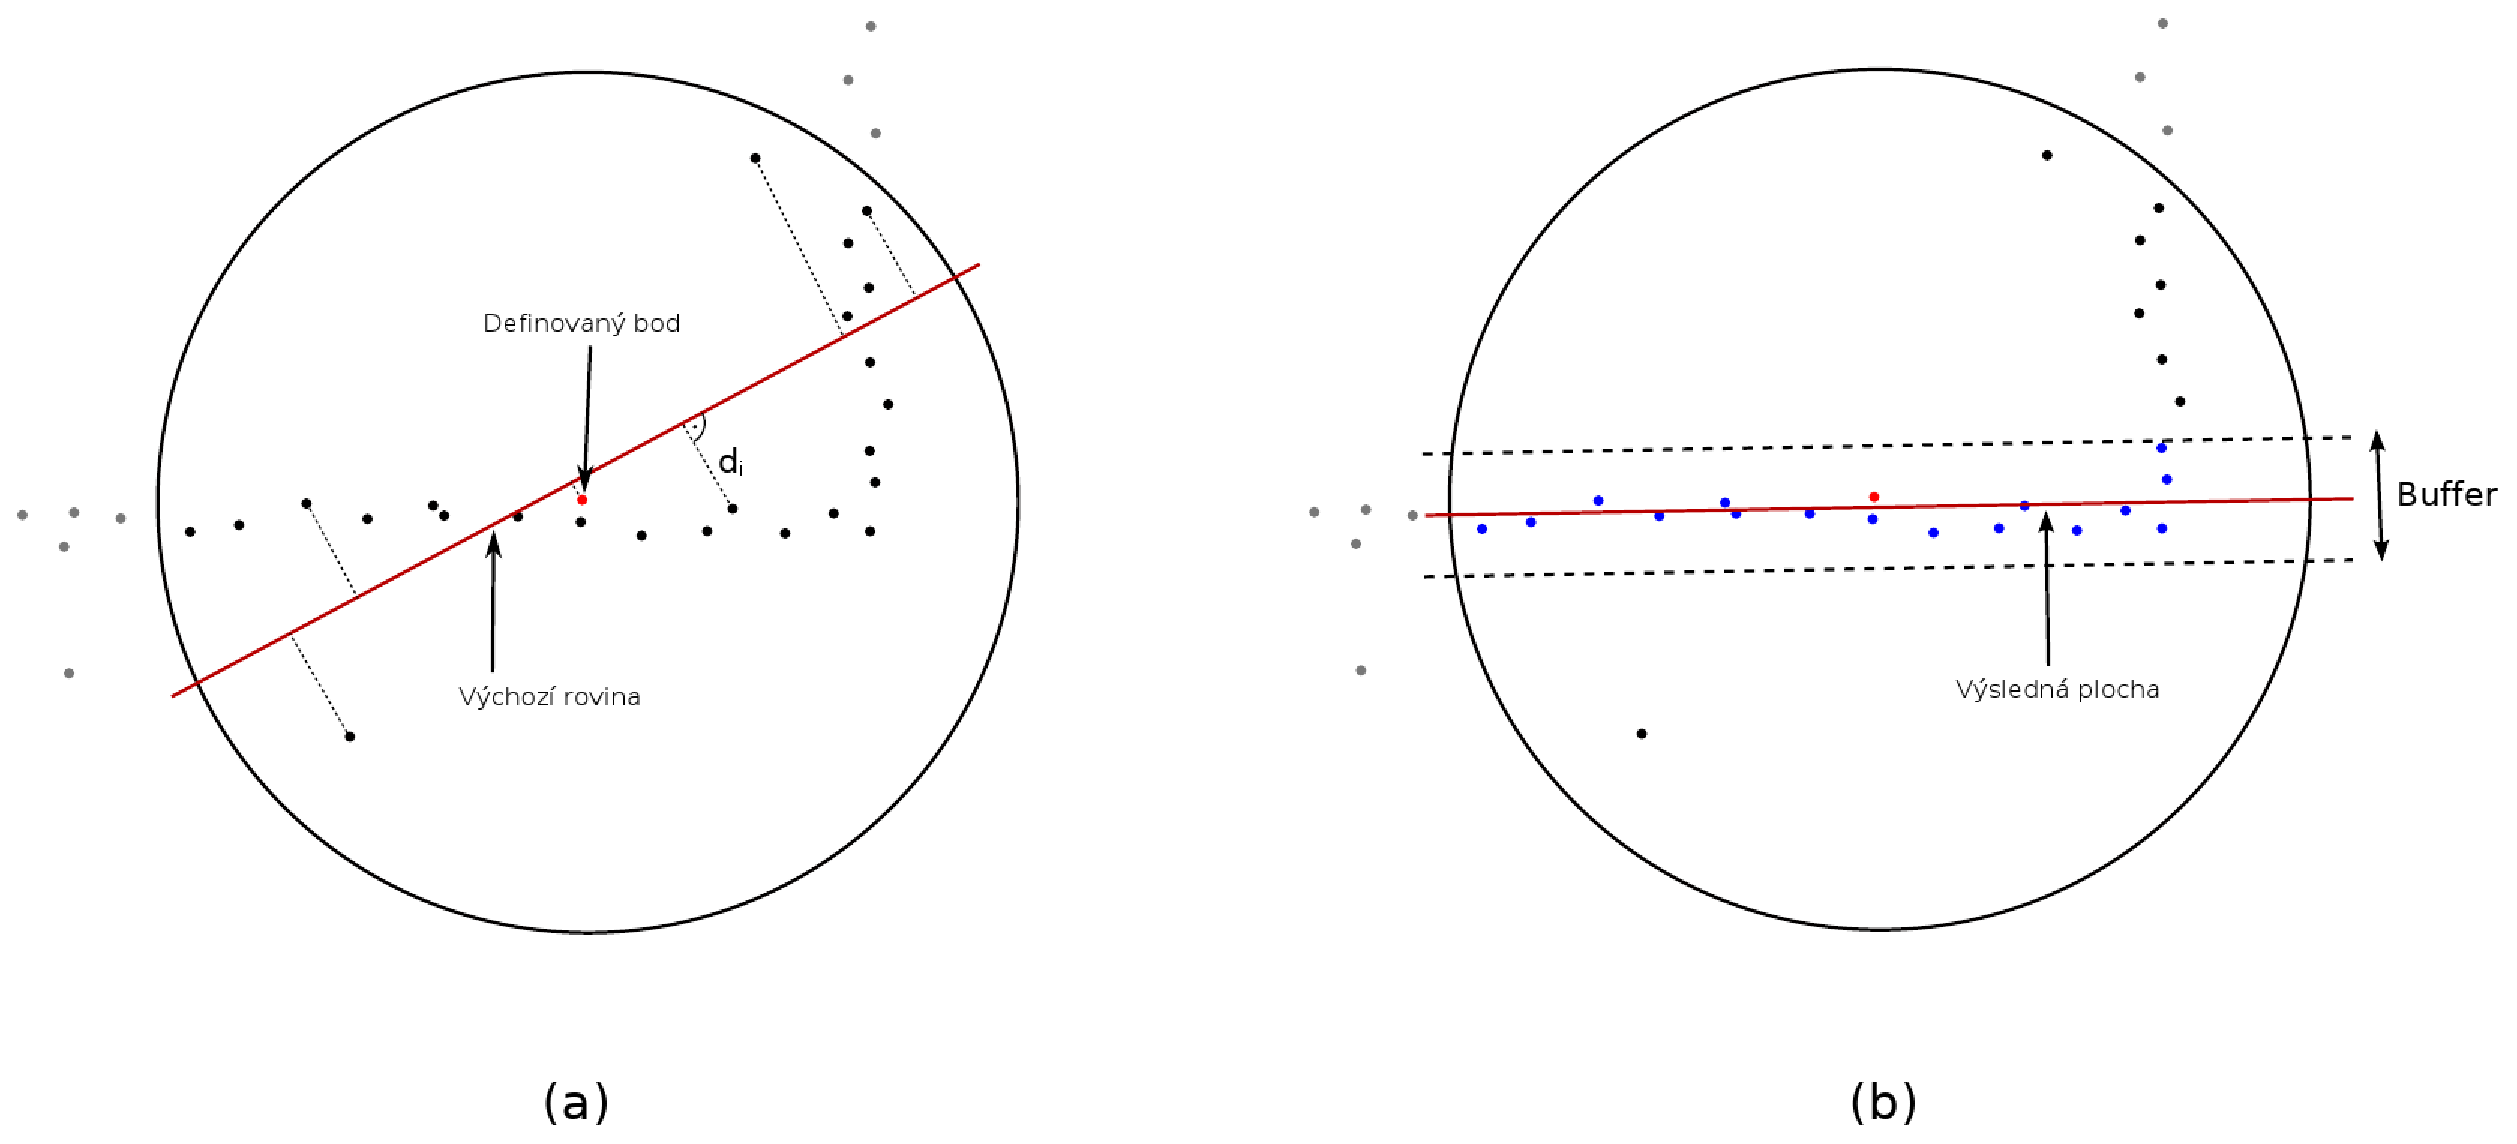
\includegraphics[width=\textwidth]{figures/2-2-definice-okoli}
\caption{Definice okolí bodu (boční pohled).\newline (a) zobrazuje proložení původní roviny body uvnitř koule. Pro některé body je znázorněna jejich váha $d_i$.\newline (b) znázorňuje výslednou rovinu po iterativním procesu, který zahrnuje váhy jednotlivých bodů. Výsledné okolí tvoří modře vyznačené body uvnitř bufferu.}
\label{fig:definice-okoli}
\end{center}
\end{figure}

Výsledné okolí se tedy nachází v útvaru, který téměř odpovídá nízkému válci, jehož osa je normála k ploše, na které se původní bod nachází. Tato osa navíc může být v průběhu algoritmu oproti výchozí hodnotě značně upravena, proto je tato metoda pojmenována adaptivní válcová definice okolí. 

\begin{figure}[htp]
\begin{center}
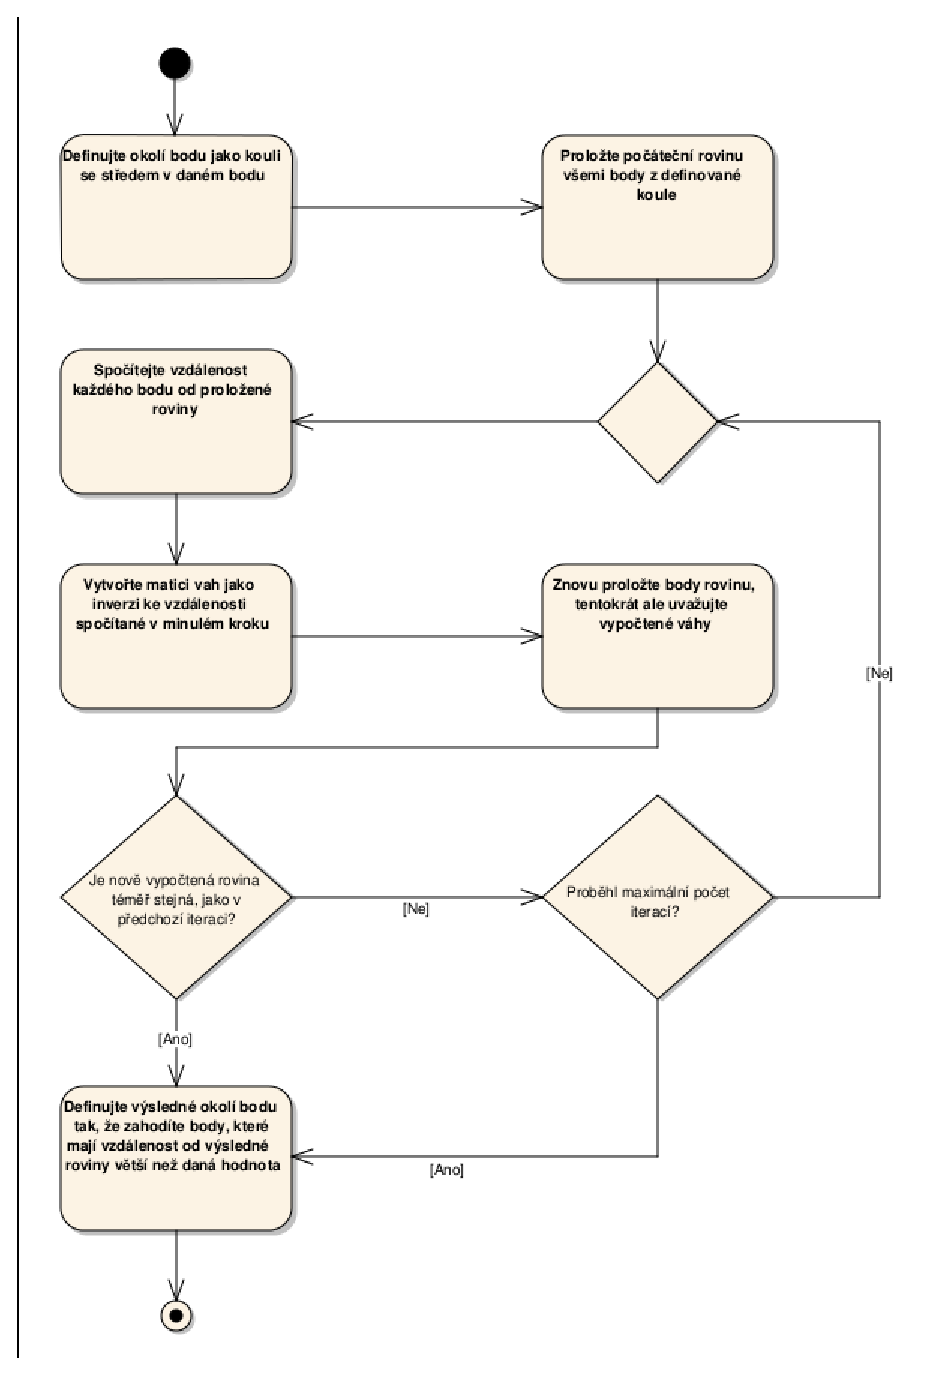
\includegraphics[width=\textwidth]{figures/2-1-okoli-diagram}
\caption{Diagram aktivit znázorňující proces definice okolí bodu.}
\label{fig:diagram-okoli}
\end{center}
\end{figure}

\newpage
\subsection{Výpočet parametrů bodu}

Atributy bodu jsou, jak již bylo zmíněno, vypočítány na základě okolí bodu. Pokud zavedeme do mračna bodů nějaký referenční bod, můžeme definovat normálový vektor z tohoto bodu na rovinu, na které se daný bod nachází. Většina metod, které provádějí klastrování na základě vypočtených parametrů, využívá hlasování do akumulátorového pole vytvořeného v prostoru parametrů. Rozměry akumulátorového pole závisí na počtu použitých parametrů. Můžeme tedy použít 3 složky normálového vektoru jako atributy a tím zajistíme, že všechny segmenty budou správně rozeznány\footnote{Mělo by být zjevné, že jeden normálový vektor jednoznačne definuje rovinu.}. Nicméně takovýto způsob vyžaduje vytvoření třírozměrného akumulátorového pole a hlasování do 3D pole je výpočetně náročná operace. 

Pro snížení výpočetních nároků je tedy nutné snížit počet parametrů. Proto je jako atribut využita velikost normálového vektoru\footnote{Myšlen je konkrétně ten normálový vektor, který začíná v daném referenčním bodu - jde tedy o vzdálenost roviny od bodu.}. Toto řešení přináší ale nebezpečí v tom, že může existovat více rovin ve stejné vzdálenosti od referenčního bodu a v takovém případě by několik rovin splynulo do jednoho segmentu. Jako řešení je zaveden druhý referenční bod a tedy i druhý atribut. Tím se značně snižuje riziko situace, kdy by více rovin mělo stejnou vzdálenost od dvou různých bodů. Obrázek \ref{fig:normal-def} (a) schématicky znázorňuje situaci, kdy mají dvě plochy stejnou vzdálenost od jednoho bodu, ale různou vzdálenost od druhého bodu, každá rovina bude mít tedy jiný pár parametrů. Na obrázku \ref{fig:normal-def} (b) jsou znározněny hlasy jednotlivých rovin zaznamenané v akumulátorovém poli. Všechny body jsou v poli zaznamenány na základě těchto dvou vypočtených parametrů. Body, které patří do různých rovin, jsou tedy v akumulátorovém poli umístěné na různých místech. Hlavní výhodou tohoto řešení je tedy to, že jsme snížili počet parametrů definujích rovinu a tím také ubrali jeden rozměr akumulátorového pole.

\begin{figure}[ht]
\begin{center}
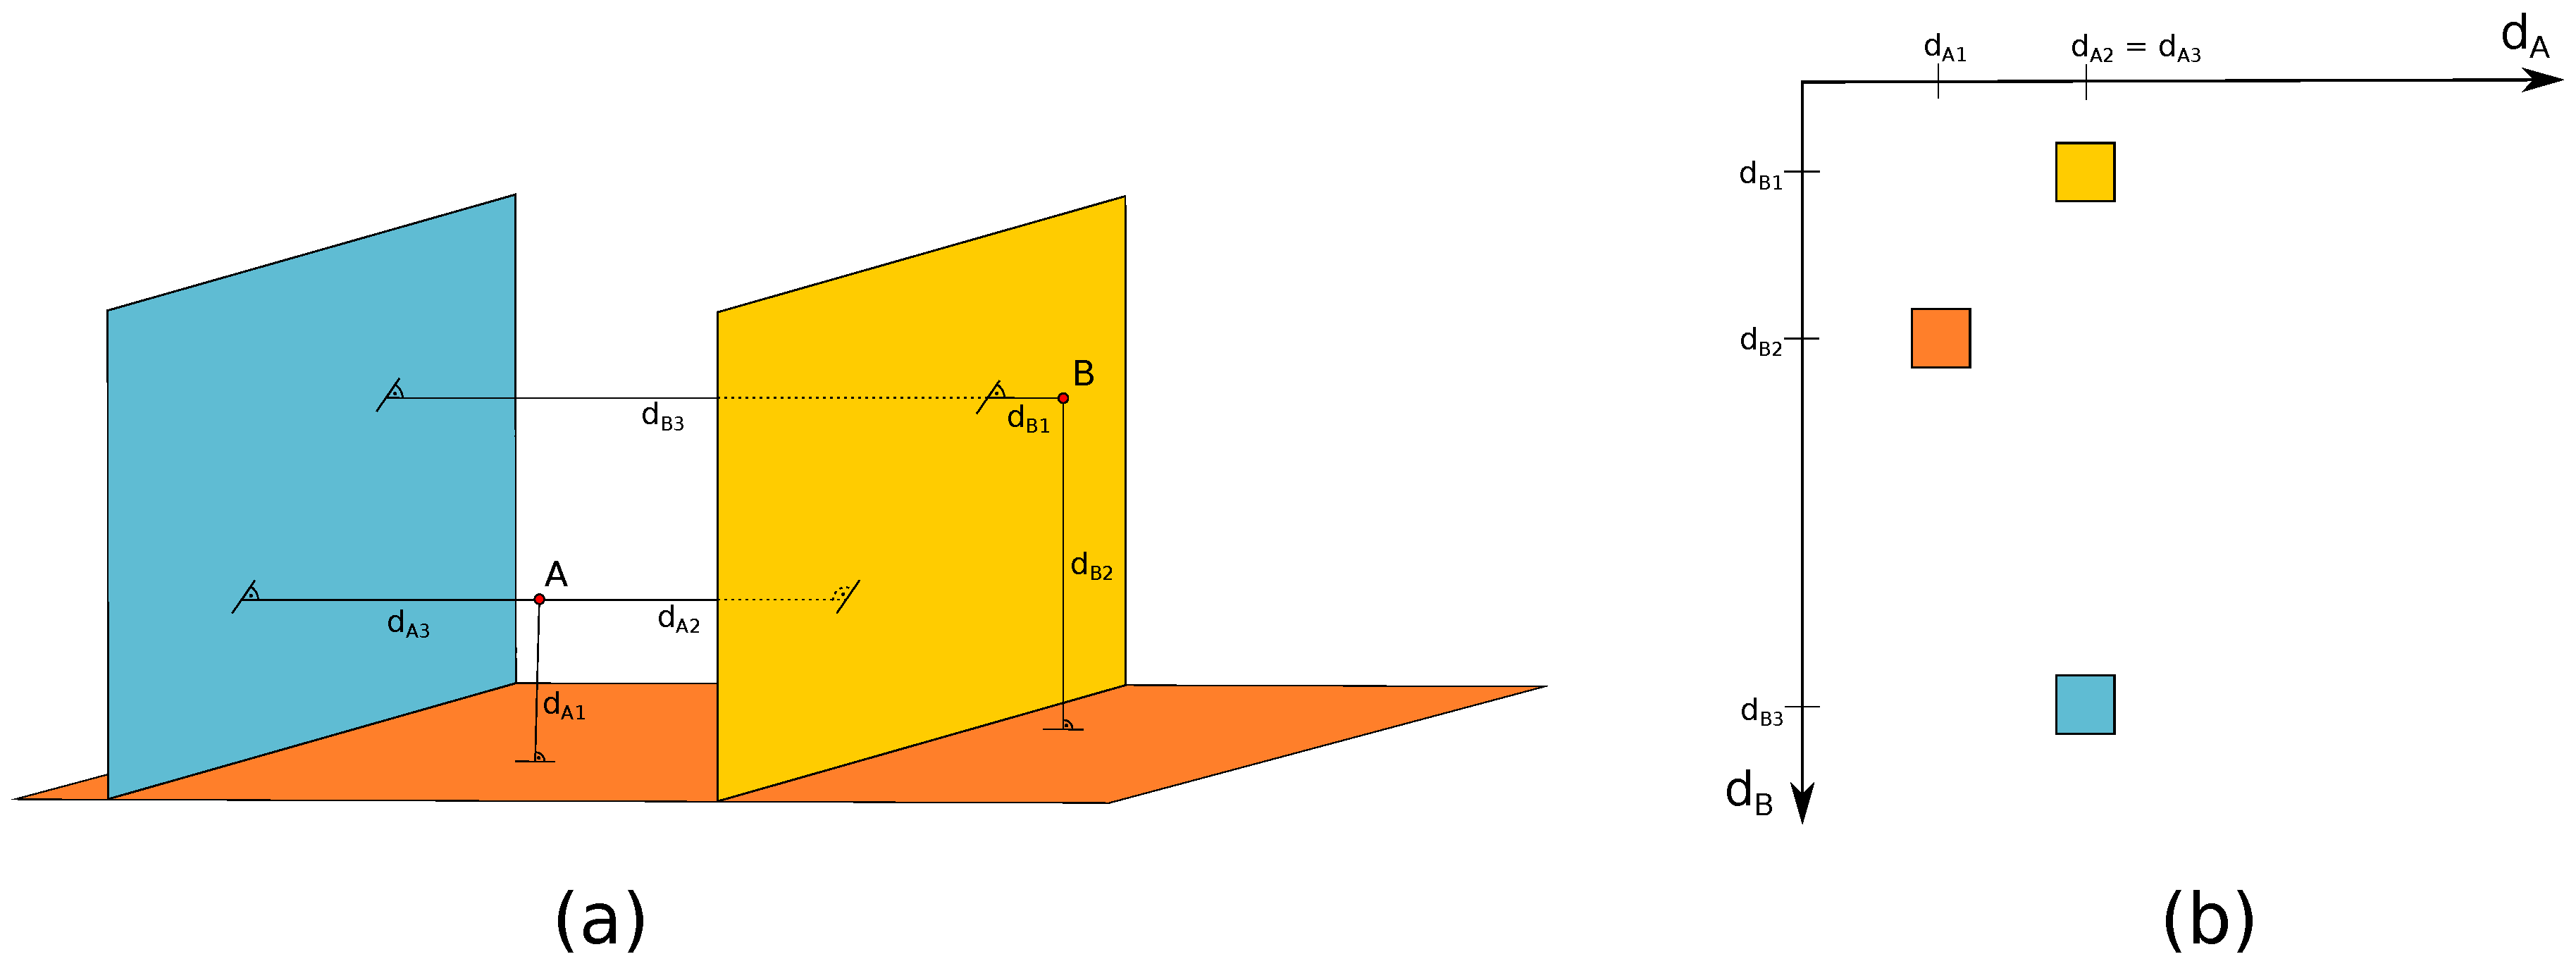
\includegraphics[width=\textwidth]{figures/definice-normal}
\caption{Schématické znároznění situace, kdy jsou dvě roviny stejně vzdálené od bodu A, ale různě vzdálené od bodu B (a), zaznamenané hlasy v akumulátorovém poli (b).}
\label{fig:normal-def}
\end{center}
\end{figure}

Důležité je tedy umístit oba referenční body tak, aby byly v datech rovnoměrně rozprostřeny. Pokud známe maximální a minimální hodnoty souřadnic v mračnu bodů, můžeme určit jejich polohu podle rovnice \ref{eq:origins}:

\begin{center}
\begin{equation} 
\label{eq:origins}
$$
referenční bod A = 
$\left( \begin{array}{ccc}
minX \\
minY \\
minZ
\end{array}\right)$ 
+ $\frac{1}{3}$
$\left( \begin{array}{ccc}
maxX - minX \\
maxY - minY \\
maxZ - minZ
\end{array}\right)$ \\
referenční bod B = 
$\left( \begin{array}{ccc}
minX \\
minY \\
minZ
\end{array}\right)$ 
+ $\frac{2}{3}$
$\left( \begin{array}{ccc}
maxX - minX \\
maxY - minY \\
maxZ - minZ
\end{array}\right)$
$$
\end{equation}
\end{center}

Umístěním referenčních bodů do těchto pozic značně snižujeme možnost, že se více rovin zobrazí na stejné místo v akuulátorovém poli. Nicméně pořád existuje možnost, že atributy dvou rozdílných rovin budou stejné nebo velmi podobné. Navíc v reálné situaci nebudou nikdy parametry všech bodů na jedné rovině stejné, ale budou v akumulátorovém poli rozptýlené ve více přilehlých políčkách. Tím se zvyšuje šance, že mohou v akumulátorovém poli dvě či více rovin splynout v jeden vrchol, který by poté byl reprezentován jako jeden segment. Proto nemůže být tato možnost ignorována a je potřeba data dále zpracovat. Tento proces detekce problému a jeho řešení je implementován v následující části, tedy v klastrování bodů.

\subsection{Klastrování bodů}

Pokud máme vypočteny pozice obou referenčních bodů, můžeme spočítat parametry všech bodů v mračnu a lužit je do akumulátorového pole. Poté může být provedeno klastrování bodů. Body, které patří do různých rovin v objektovém rostoru, vytvoří různé vrcholy v prostoru parametrů. Na obrázku \ref{fig:acc-pole} je znázorněn příklad takové situace. Mračno bodů, které obsahuje tři kolmé roviny, vytvoří pomocí hlasování v akumulátorovém poli tři různé vrcholy.

\begin{figure}[ht]
\begin{center}
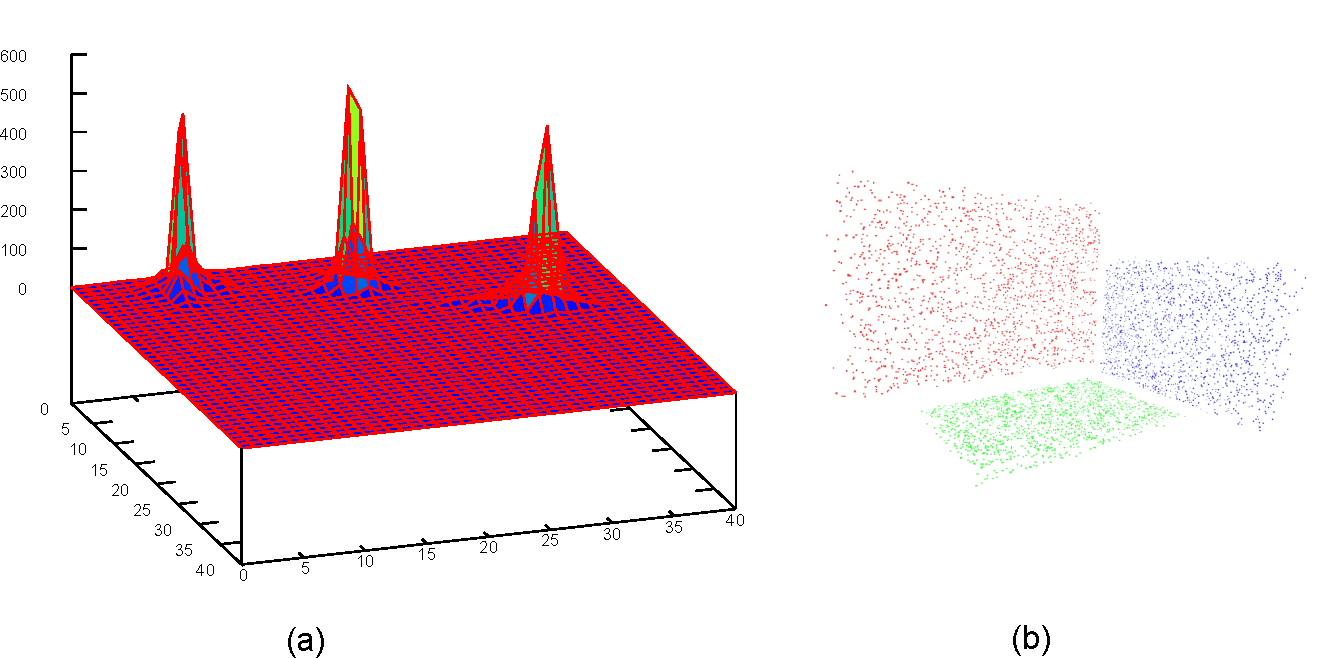
\includegraphics[width=\textwidth]{figures/ac-pole}
\caption{Ukázka akumulátorového pole (a), které representuje mračno bodů se třemi kolmými rovinami (b). Svislá osa grafu reprezentuje počet bodů, vodorovné osy parametry bodů (tedy souřadnice v poli).}
\label{fig:acc-pole}
\end{center}
\end{figure}

Pokud máme všechny body uloženy v akumulátorovém poli, vyhledáme buňku s největším počtem bodů (tedy nejvyšší vrchol). Velikost buňky v akumulátorovém poli je určena na základě velikosti šumu ve vstupním mračnu. Tyto body z nejvyššího vrcholu proložíme rovinou pomocí metody nejmenších čtverců. Poté ohodnotíme kvalitu roviny výpočtem efektivní hodnoty (dále jen EH) vzdáleností všech bodů od proložené roviny. Pokud máme množinu $n$ bodů $\left\{x_1, x_2, \ldots , x_n\right\}$ a jejich vzdáleností od proložené roviny $\left\{d_1, d_2, \ldots , d_n\right\}$, vypočítáme EH podle vztahu \ref{eq:rms}:

\begin{equation} 
\label{eq:rms}
eh = \sqrt{
\frac{1}{n}\left({d_1}^2 + {d_2}^2 + \ldots + {d_n}^2\right)
}
\end{equation}

Přijatelná hodnota je závislá na velikosti šumu v datech, obecně lze říct, že kvalita roviny je dostatečná, pokud je vypočtená EH menší, než velikost šumu v datech. Pokud je EH větší, pravděpodobně jsme detekovali výše popsaný problém, kdy více rovin splynulo v akumulátorovém poli do jednoho segmentu. Řešení tohoto problému bude popsáno ke konci této sekce.

Pokud je tedy vypočtená EH v přijatelných mezích, vytvoříme počáteční klastr, do kterého dáme všechny body dané buňky. Klastrování pokračuje body, které do této buňky nepatří, ale jsou v jejím okolí. Tento krok je nezbytný, protože data obvykle nebývají tak přesná, aby se všechny body z roviny trefily přesně na jedno místo v akumulátorovém poli, zejména jde o body v okolí hran. Tento postup probíhá iterativně a funguje tak, že v první iteraci je identifikováno 8 buňek v sousedství buňky s největším počtem bodů (viz Obr. \ref{fig:acc-pole-clus}).  Body z těchto osmi buněk přidáme do segmentu pouze, pokud splní dvě podmínky. První podmínkou je, že bod musí být prostorově blízko k bodům z původního klastru (např. 2x průměrná vzdálenost mezi body v původním klastru). Poté je spočítána vzdálenost bodů od roviny, která je definována body z původního clusteru. Pouze body, které jsou blíže, než je předem daný práh, mohou být přidány do klastru. Tento práh je opět určet v závislosti na velikosti šumu v datech.  Body, které nesplnily jednou z těchto dvou podmínek zůstanou na své pozici v akumulátorovém poli a jsou znovu posouzeny v dalších iteracích. Pokud jsou do klastru přidány všechny body, které splňují obě podmínky, přepočítají se parametry klastru - tedy opět se body proloží rovina, ale jsou zahrnuty i nově přidané body. Poté proces pokračuje druhou iterací. V té jsou procházeny body z 24 sousedních buněk (viz Obr. \ref{fig:acc-pole-clus}). Proces je navržen tak, aby v této iteraci byly opět procházeny i ty body, které neprošly podmínkami v první iteraci. Protože se na konci každé iterace přepočítavají parametry, mohou být tyto body v dalších iteracích do klastru zahrnuty. Takto iterativně proces pokračuje až do té doby, než do klastru nemohou být přidány žádné nové body. V tu chvíli je klastr zaznamenán a všechny jeho body jsou odebrány z akumulátorového pole.

\begin{figure}[ht]
\begin{center}
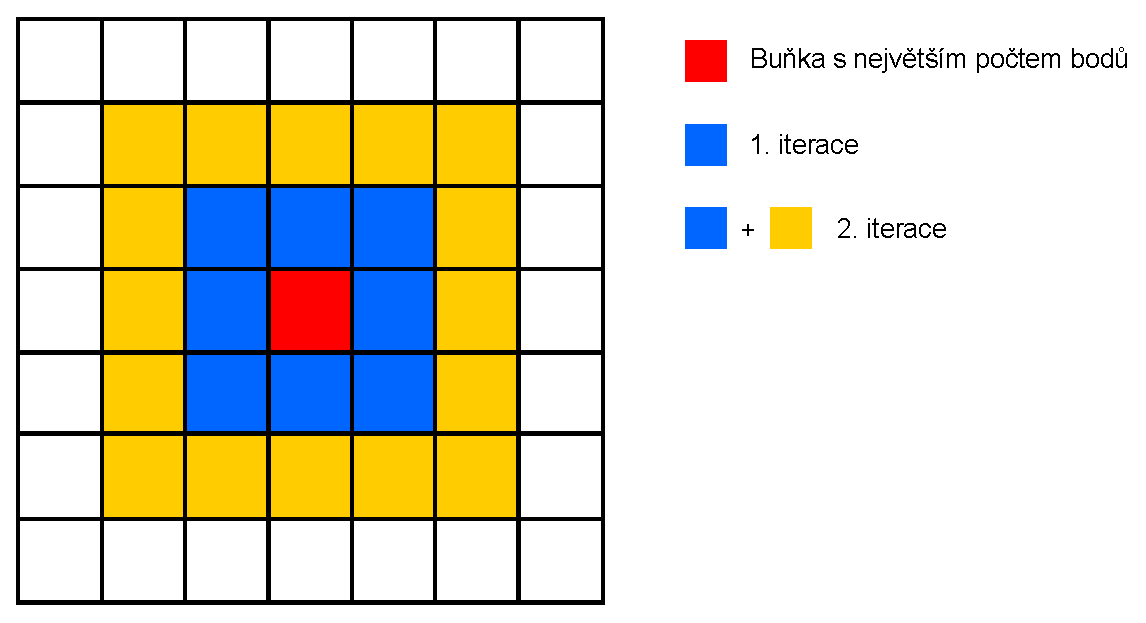
\includegraphics[width=12cm]{figures/acc-pole-clustering}
\caption{Prohledávání políček v akumulátorovém poli v průběhu jednotlivých iterací.}
\label{fig:acc-pole-clus}
\end{center}
\end{figure}

Nyní proces pokračuje k druhému nejvyššímu vrcholu v akumulátorovém poli, který je nalezen stejným způsobem, jako byl ten nejvyšší v předchozí iteraci. Poté se opakují stejné kroky, jako v předchozím případě. Celý tento proces přesouvání se od nejvyššího vrcholu k druhému nejvyššímu pokračuje až do té doby, dokud je velikost nejvyššího vrcholu větší, než předdefinovaná hranice.

Poslední součástí algoritmu je řešení situace, kdy více rovin sdílí stejný vrchol v akumulátorovém poli. Tuto situaci jsme již detekovali pomocí výpočtu EH. Pokud je vypočetná EH příliš vysoká, s velkou pravděpodobností jsou ve vrcholu body z více různých rovin. V takovém případě jsou definovány dva nové referenční body. Pozice nových referenčních bodů je definovaná podle vztahu \ref{eq:new-origins}:

\begin{center}
\begin{equation} 
\label{eq:new-origins}
$$
$\left( \begin{array}{ccc}
X_n \\
Y_n \\
Z_n
\end{array}\right)$ = 
$\left( \begin{array}{ccc}
X_o \\
Y_o \\
Z_o
\end{array}\right)$ 
+ 
$\left( \begin{array}{ccc}
range \times rand \\
range \times rand \\
range \times rand
\end{array}\right)$
$$
\end{equation}
\end{center}

kde ($X_n$, $Y_n$, $Z_n$) jsou souřadnice nového bodu, ($X_o$, $Y_o$, $Z_o$) jsou souřadnice původního bodu, $range$ je hodnota určující jak nejdál může být nový bod posunut (např. 5m) a $rand$ je náhodná hodnota z intervalu (0,1).

Poté je definováno malé akumulátorové pole pouze pro tyto body (způsobující problém) a na základně nově definovaných referenčních bodů jsou přepočteny atributy bodů. Poté jsou vyhledány nově vytvořené vrcholy a ty jsou klastrovány stejným způsobem, jako v běžném případě. tento proces se opakuje do té doby, než jsou nalezeny dostatečně kvalitní roviny. V případě, že do určitého počtu iterací (např. 10) není nalezena žádná přijatelná rovina, vezme se druhá nejvyšší buňka ze zpracovávaného vrcholu v původním poli, proloží se rovinou a ohodnotí se její kvalita výpočtem EH. Poté proces pokračuje standardně jednotlivými kroky, které již byly popsané.

Tímto jsme popsali celý algoritmus. Jak by mělo být patrné, algortimus bere v úvahu vztahy bodů v prostoru parametrů a zároveň jejich vzdálenost v prostoru. navíc je tento algoritmus poměrně robustní, protože při klastrování mají prioritu body, které mají podobnější parametry a zároveň jsou blízko v prostoru, před body, jejichž parametry jsou více odlišné.


\section{Segmentace pomocí vyhledávání dominantních os}

\cite{Seg02}


\section{Proložení roviny množinou bodů}
\label{sub:lsq}
Důležitou součástí prvního algoritmu je proložení roviny množinou bodů pomocí metody nejmenších čtverců, viz \cite{wiki:leastsq}. Předpoklad tedy je, že chceme nalézt rovinu, která je co nejblíže od všech 3D bodů z dané množiny. Mějme množinu velikosti $k$, která obsahuje body ($p_1, \ldots, p_k$). Rovina je definována bodem $c$, který leží v rovině, a normálový vektorem $n$. Pro libovolný bod $x$ ležící v rovině platí vztah $n(x - c)^T = 0$. Pokud vezmeme bod $y$, který v rovině neleží, potom platí $n(y - c)^T \neq 0$. Je tedy vhodné definovat odchylku podle vztahu \ref{eq:odchylka}:

\begin{equation}
\label{eq:odchylka}
(n (p_i - c)^T)^2
\end{equation}

Proložená rovina má být co nejblíže ke všem bodům. Hledáme takové $n$, které minimalizuje celkovou odchylku všech bodů. Rovinu tedy můžeme získat vyřešením následujícího vztahu:

\begin{equation}
\label{eq:ls-min}
\min_{c,\|n\|=1} \sum\limits_{i=1}^k (n (p_i - c)^T)^2
\end{equation}

Řešení tohoto vztahu pro $c$ je:

\begin{equation}
c = \frac{1}{k} \sum\limits_{i=1}^k p_i
\end{equation}

Bod $c$ je tedy aritmetickým průměrem všech prokládaných bodů (pro tento bod se používá označení centroid). Pokud si definujeme matici $M$, která má v $i$-tém řádku hodnoty $p_i - c$ (jde tedy o matici $k \times 3$), můžeme vztah  \ref{eq:ls-min} přepsat do této formy:

\begin{equation}
\min_{\|n\|=1} \|M n\|^2
\end{equation}

Řešením tohoto problému je SVD dekompozice matice $M = USV^T$, kdy vektor $n$ je určen pravým singulárním vektorem matice $M$, který odpovídá nejmenší singulární hodnotě. Konkrétně jde o poslední sloupec matice $V^T$.

Pokud tedy máme vypočtený bod $c$ a normálový vektor $n$, můžeme snadno vyjádřit rovinou např. obecnou rovnicí:

\begin{equation}
ax + by + cz + d = 0
\end{equation}

ve které parametry $a, b, c$ jsou složky normálového vektoru $n$ a $d$ spočteme jednoduše dosazením bodu $c$:

\begin{equation}
\label{eq:d}
d = -(n_1c_1 + n_2c_2 + n_3c_3)
\end{equation}

Toto řešení předpokládá, že všechny body mají stejnou váhu. Pokud máme pro body různé váhy, do výpočtu je zahrneme poměrně jednoduše. Pokud má bod $p_i$ váhu $w_i$, musíme vztah \ref{eq:ls-min} upravit tímto způsobem:

\begin{equation}
\min_{w_i,c,\|n\|=1} \sum\limits_{i=1}^k w_i (\times n (p_i - c)^T)^2
\end{equation}

Stejně musíme upravit definici matice $M$, která bude v každém řádku obsahovat hodnoty $w_i \times (p_i - c)$. Ostatní postup však zůstává stejný.

%*****************************************************************************
\chapter{Implementace}

Tato kapitola se zabývá popisem implementace obou algoritmů. Algoritmy jsou implementovány v jazyce Java v rámci dodaného softwaru ArchiRec3D \cite{AR3D}. Kompletní zdrojový kód je k dispozici na přiloženém CD, viz kapitla~\ref{chap:CD}.

\section{Segmentace na základě velikosti normálového vektoru}

Implementaci tohoto algoritmu můžeme rozdělit na dvě hlavní části. První částí je výpočet parametrů pro všechny body a uložení bodů do akumulátorového pole. Druhou částí bude poté klastrování bodů v akumulátorovém poli. Tyto dvě části budou reprezentovány jako samostatné metody. První metoda bude mít na vstupu zpracovávané mračno bodů a jejím výstupem bude akumulátorové pole naplněné všemy body ze vstupního mračna. Druhá metoda bude mít toto akumulátorové pole na vstupu a výstupem budou body rozdělené do jednotlivých sementů. Takovéto rozdělení má hlavní výhodu v tom, že obě části budou na sobě nezávislé. Bude tedy možné jednou uložit body do akumulátorového pole a poté provést klastrování několikrát s různými parametry bez nutnosti znovu provádět první část.

\subsection{Uložení bodů do akumulátorového pole}

Tato část algoritmu bude procházet všechny body, na základě jejich okolí bude vypočítávat parametry, podle kterých budou body uloženy do akumulátorového pole. Vstupem bude tedy mračno bodů a výstupem akumulátorové pole. Prvním problémem bude tedy to, jak v paměti správě reprezentovat obě tyto struktury. To se samozřejmě musí odvíjet od operací, které budeme s daty provádět. Protože algoritmus implementuji v rámci dodaného nástroje, mám k dispozici několik základních datových struktur jako např \verb|vicitis.inner.Point3D| pro reprezentaci 3D bodu, \verb|vicitis.inner.Plane3D| pro reprezenatci roviny apod., tak samozřejmě tyto datové struktury využiji. Navíc je zde také implementováno mnoho vhodných metod využívajících tyto třídy, takže je logické použít již funkční řešení a nevymýšlet vlastní, které by bylo navíc duplicitní.

Základním požadavkem na datovou strukturu reprezentující mračno bodů je možnost vyhledávat sousední body v 3D prostoru. Protože tuto operaci je nutné provádět pro každý bod, je důležité, aby byla tato operace co nejrychlejší. Naopak vytváření struktury se bude provádět pouze jednou a už do ní nebudeme za běhu přidávat ani odebírat body, takže na tyto operace nemusí být kladeny velké nároky. Pro tyto účely se nejčastěji využívají stromy, které umožňují rekurzivní dělení n-dimenzionálního prostoru na menší podprostory. Jedním z takovýchto algoritmů je octree, který rekurzivně dělí prostor na 8 podprostroů. Podobný algoritmus je kd-strom \cite{wiki:kdtree}, kde jednotlivé uzly jsou k-dimenzionální body. Tento typ stromu dělí prostor na podprostory podél těchto jednotlivých dimenzí. Pokud srovnáme tyto dva algoritmy, tak octree se rychleji staví a zároveň umí jednoduše přidávat nové body do již postaveného stromu. Oproti tomu do kd-stromu se body za běhu přidávají mnohem složitěji, ale algoritmus je efektivnější pro vyhledávání bodů a nejbližších sousedů. Protože jsem určil rychlé vyhledávání nejbližších sousedů jako nejdůležitější kritérium, vybral jsem nakonec pro reprezentaci mračna bodů kd-strom. Vyhledání nejbližšího souseda v kd-stromu (o $n$ prvcích a $k$ dimenzích) má v nejlepším případě asymptotickou složitost $O(log~n)$ a v nejhorším případě $O(k \times n^{1-\frac{1}{k}})$, ve většině případů má však složitost blíže k nejlepšímu případu. Podrobný popis kd-stromu je k dispozici v \cite{wiki:kdtree}. Samozřejmě implementace kd-stromu je poměrně složitá, obzvláště, pokud má být co nejefektivnější. Proto jsem se rozhodl pro použití knihovny. Po vyzkoušení několika různých knihoven byla jednoznačně nejrychlejíší implementace \cite{kdtree}, kterou jsem použil.

Pro akumulátorové pole potřebujeme nějaké dvourozměrné pole, které nám bude udržovat body  s danými parametry na jednotlivých pozicích v poli. Bylo by možné použít obyčejné \verb|int[][]| pole, které by pouze ukládalo počet bodů na jednotlivých políčkách. Takové řešení by na první pohled mohlo pro vyhledávání vrcholů při klastrování dostatečné, nicméně by bylo výpočetně náročné zpětně zjistit, které body na dané pozici jsou. Proto bude jednodušší, když budou body uložené přímo v akumulátorovém poli. Proto jsem zvolil 2D pole seznamů \verb|ArrayList<Point3D>[][]|, které bude udržovat body na jednotlivých políčkách pole. Takto budu při vyhledávání vrcholů v poli jednoduše vědět, kolik bodů se na daném políčku nachází, ale zároveň půjde tyto body ihned zpracovávat bez dalšího vyhledávání. 

Velmi důležité jsou také rozměry akumulátorového pole. Podle teorie je buňky v akumulátorovém poli určena na základě velikosti šumu ve vstupním mračnu. Bohužel testovací data, která mám k dispozici, nemají šum definovaný. Proto je nutné vymyslet vlastní strategii pro určení velikosti akumulátorového pole. Pokud je akumulátorové pole příliš malé, jednotlivé vrcholy mohou splynout, nepůjde je v poli detekovat a algoritmus prakticky nebude funkční. Pokud naopak bude akumulátorové pole příliš velké, vrcholy v poli nebudou výrazné a výsledek bude stejný jako v předchozím případě - algoritmus nebude fungovat tak, jak by se od něj čekalo. Původně jsem vycházel z úvahy, že velikost políčka v akumulátorovém poli bude např. jedna tisícina z velikosti mračna bodů. V takovém případě je ale velikost pole pro všechny vstupní data stejná (např. $1000~\times~1000$). To ale není vhodné řešení, protože vstupní data mohou obsahovat řádově tisíce až miliony bodů a nezdá se logické, aby pro oba případy bylo akumulátorové pole stejně velké (a v praxi se to také ukázalo jako nefunkční řešení). Z toho jsem tedy usoudil, že velikost akumulátorového pole bude výrazně závislá na počtu vstupních bodů. Proto se zdá rozumné odvodit velikost pole právě od této hodnoty. Nejprve jsem zkusil určit velikost jako tisícinu z počtu bodů. To se také neukázalo jako vhodné řešení, protože pro malá mračna bylo pole příliš malé a pro velká mračna naopak příliš velké (pro 1,5 milionu bodů by bylo potřeba alokovat pole o rozměrech $15000~\times~15000$, což by bylo paměťově extrémně náročné). Lineární závislost mezi počtem bodů a velikostí akumulátorového pole tedy není správné řešení. Došel jsem tedy k úvaze, že by mohla být vhodná volba stejný počet políček v akumulátorovém poli, jako je počet bodů. To nám zajistí, že pole nikdy nebude příliš malé, protože se předpokládá, že body na stejné ploše budou jen v několika sousedních políčkách. Proto by mělo v poli zbýt dostatek volných políček, aby jednotlivé vrcholy nesplynuly dohromady. Po vyzkoušení na reálných datech jsem zjistil, že velikost pole není ani příliš velká a vrcholy jsou dostatečně rozeznatelné. Jako rozměr akumulátorového pole jsem tedy určil odmocninu z počtu bodů (to odpovídá stavu, že počet políček v poli se rovná počtu bodů). V takovém případě je pro mračno s 10 tisíci body alokováno pole velikosti $100~\times~100$, pro 1,5 mil bodů je to pole o rozměrech $1225~\times~1225$. Samozřejmě ani toto není optimální řešení. Velikost pole by měla být nejlépe odvozena od konkrétního zpracovávaného mračna a jeho vlastností jako očekávaný počet rovin, hustota bodů, počet bodů mimo roviny apod. Nicméně takový algoritmus by nebyl vůbec jednoduchý a pravděpodobně by vyžadoval nějaké vstupní parametry zadané uživatelem. To je ale nevhodné, za prvé se očekává, že algoritmus bude co nejvíce automatický, za druhé by běžný uživatel bez hlubších znalostí nebyl schopen takové parametry zadat. Proto jsem nakonec zvolil výše popsané řešení.

Nyní máme připravené potřené datové struktury, můžeme tedy začít se samotným algoritmem. Nejprve si tedy vytvoříme novou instanci kd-stromu, konkrétně instanci třídy \verb|SqrEuclid|, což je kd-strom, který využvívá klasickou euklidovskou vzdálenost mezi body. Poté kd-strom  v cyklu naplníme body a zároveň získáme jednoduchým porovnáním  největší a nejmenší hodnoty součřadnic v celém mračnu bodů. Tyto souřadnice využijeme k výpočtu pozic referenčních bodů podle vztahu \ref{eq:origins}.

Ještě před samotným výpočtem parametrů bodů musíme stanovit velikost koule, která definuje okolí (viz sekce \ref{sub:def-okoli}). V popisovaném algoritmu je tato velikost popisována euklidovskou vzdáleností (např. 3m). Já ale v testovacích datech žádné měřítko nemám, navíc mně dostupná data jsou poměrně odlišná od dat, které používali v článku. Proto je tato definice nevhodná a je potřeba ji nějak obejít. Protože mohou mít různá data výrazně jinou hustotu bodů, přijde mi rozumné velikost koule vypočítat z daného konstatního počtu bodů. Bohužel určit tento počet naprosto obecně pro libovolný typ dat je téměř nemožné. Proto jsem se rozhodl nechat tuto hodnotu jako volný parametr, který bude zadán uživatelem. To má i další důvod, tato hodnota velmi zásadně ovlivňuje dobu běhu algoritmu. Vyhledávání okolí v kd-stromu je drahá operace a pokud se pro každý bod vyhledává okolí v řádu stovek bodů, algoritmus může běžet desítky minut, což jistě není vždy optimální. Zároveň ale do určité míry platí, že čím větší okolí bodu se bere v úvahu, tím přesnější jsou vypočtené parametry bodu. Tím, že nechávám tento parametr na uživateli, mu dávám možnost vybrat si mezi rychlostí nebo kvalitou. Pokud tedy zadám malé hodnoty tohoto parametru, např. 10 - 50, tak je algoritmus poměrně rychlý, ale může dávat horší výsledky. Pokud zadám větší hodnoty, např. 80 - 200, tak může být doba běhu algoritmu výrazně pomalejší, zato s kvalitnějšími výsledky. Obecně bych doporučil volit hodnoty z intervalu 20 - 200 s tím, že vhodný kompromis mezi kvalitou a rychlostí je 40 - 80. Konkrétní dopad těchto hodnot na dobu běhu a kvalitu segmentace bude popsán v kapitole \ref{chap:test}. Je důležité zmínit, že tato hodnota se musí odvíjet zejména od vstupních dat, nikoliv pouze od toho, zda chceme kvalitu nebo výkon. Pokud máme data hodně přesná (tedy body v rovině mají od této roviny jenom minimální odchylku), můžeme volit menší hodnoty pro velikost okolí a výsledek bude stále kvalitní. Pokud máme ale např. data reprezentující budovu s taškovou střechou (obecně s nerovným povrchem), kterou chceme rozpoznat jako sement, musíme volit okolí větší. Na obrázku \ref{fig:strecha} je ukázka takové situace, kdy volba příliš malého okolí značně ovlivní výsledný výpočet.

\begin{figure}[ht]
\begin{center}
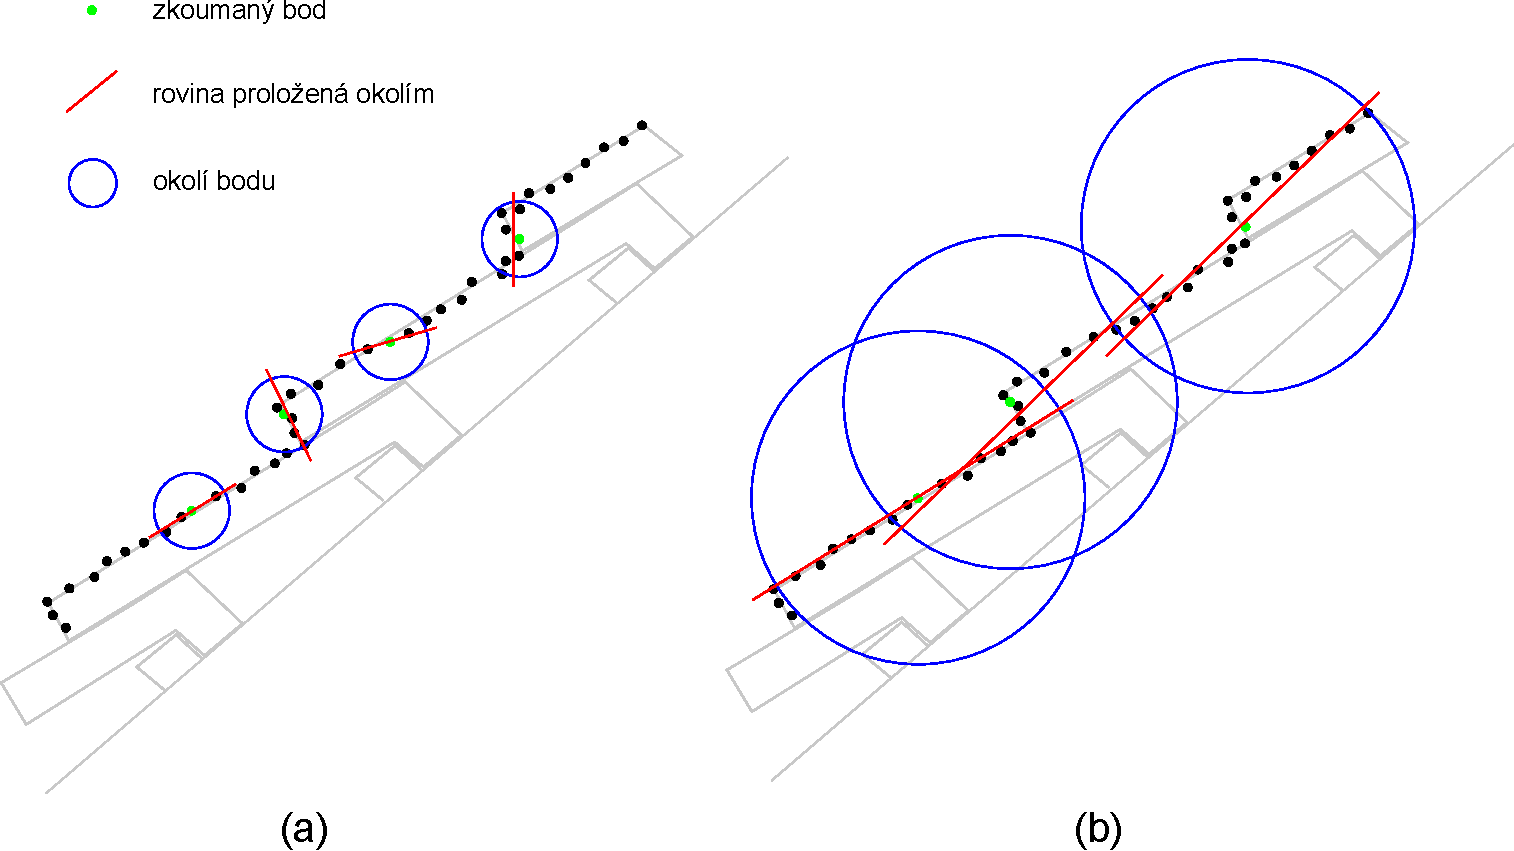
\includegraphics[width=\textwidth]{figures/strecha-all}
\caption{Ukázka vlivu velikosti okolí na vypočítávané parametry. Malé okolí může způsobit chybný výpočet (a), oproti tomu velké okolí je přesnější (b).}
\label{fig:strecha}
\end{center}
\end{figure}

Hodnota, kterou uživatel zadá se ještě přímo nevyužije k definici okolí. Tato hodnota se využije pouze k vypočtení velikosti výsledné koule. Výpočet probíhá tak, že se náhodně vybere z mračna určitý počet bodů (např. setina ze všech bodů). Pro každý náhodně vybraný bod se vybere takový počet nejbližších sousedů, jaká je hodnota zadaného parametru. Poté se spočítá poloměr koule, které vybrané body tvoří (tedy vzdálenost střed - nejvzdálenější bod). Nakonec se spočítá aritmetický průměr všech vypočtených poloměrů. Tento aritmetický průměr je konečná velikost koule, která bude v algoritmu definovat okolí bodu. Pro všechny body bude mít tedy okolí stejnou velikost, ale bude pokaždé obsahovat různý počet bodů.

V tuto chvíli již máme všechny potřebné informace pro výpočet parametrů všech bodů. Máme načtené body v kd-stromu, máme definované oba referenční body, dále máme vypočtenou velikost koule pro okolí bodu a máme připravené akumulátorové pole, do kterého budeme body ukládat. Vytvoříme tedy cyklus, pomocí kterého budeme procházet všechny body v mračnu.

Nyní potřebujeme pro každý bod získat jeho okolí, tedy všechny body, které leží v kouli se středem v daném bodu a poloměrem, který jsme vypočítali. Víme, kolik by mělo být v této kouli průměrně bodů. Pro první iterovaný bod tedy vezmeme tento počet nejbližích sousedů. Vyhledávání n nejbližších sousedů je v kd-stromu definovaná operace, takže je to velmi jednoduché. Dále si spočítáme vzdálenost definovaného bodu a nejvzdálenějšího bodu z vybraných sousedů (kd-strom vrací body seřazené podle vzdálenosti od původního bodu, takže nejvzdálenější bod je ten poslední v seznamu). Pokud je tato vzdálenost větší, než je velikost koule definující okolí, tak pomocí binárního prohledávání projdeme seznam sousedů a nalezneme nejvzdálenější bod, který ještě leží uvnitř koule. Všechny body, které jsou dál, zahodíme. Pokud nastane situace, kdy ještě nemáme dostatek bodů, vynásobíme aktuální počet vybraných sousedů $1,5 \times$ a tento nový počet opět vybereme z kd-stromu a testujeme. Takto pokračujeme do té doby, než máme dostatek bodů. Je potřeba zmínit, že tento iterativní proces by měl nastat co nejméně, protože vyhledávání nejbližších sousedů v kd-stromu je pomalá operace. Celý výše popsaný proces získávání bodů pro okolí je přehledně znázorněn na diagramu \ref{fig:diag-okoli}.

\begin{figure}[ht]
\begin{center}
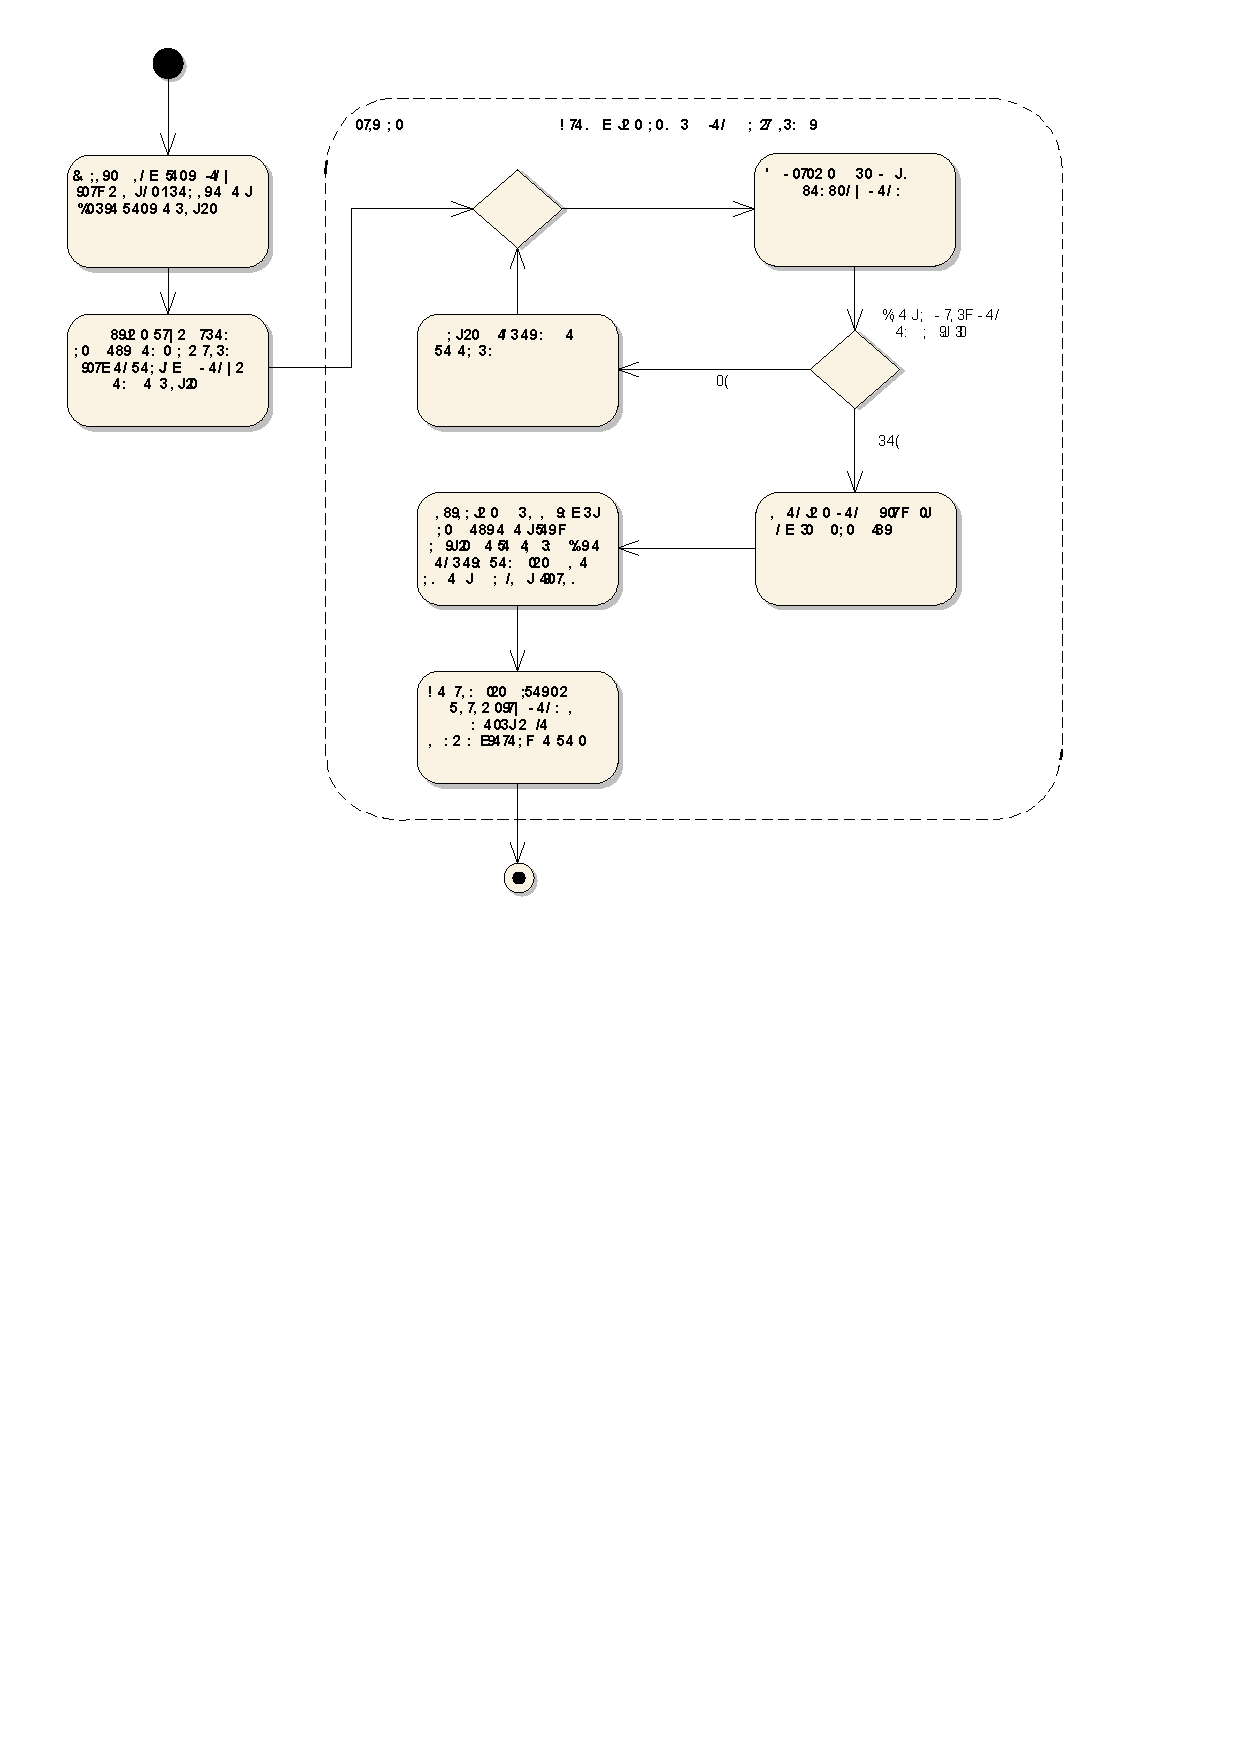
\includegraphics[width=\textwidth]{figures/okoli-diagram-algoritmus}
\caption{Diagram znázorňující získání potřebných nejbližších sousedů bodu.}
\label{fig:diag-okoli}
\end{center}
\end{figure}

Protože blízké body v mračnu bodů budou mít pravděpodobně velmi podobné okolí, využijeme výslednou velikost okolí jako výchozí hodnotu pro bod v další iteraci. Tady nastává otázka, jestli použít přesně tu samou hodnotu nebo jí o trochu zvýšit. Vyhledávání bodů v kd-stromu je pomalá oprace a nechceme, aby bylo v další iteraci zbytečně provedeno dvakrát, protože chybělo několik málo bodů. Zároveň je ale nutné vzít v úvahu, že čím více bodů v kd-stromu vyhledáváme, tím pomalejší toto vyhledávání je. Je tedy otázka, jaký je optimální poměr navýšení počtu bodů do další iterace. Proto jsem se rozhodl určit tento parametr experimentálně. Porovnal jsem 3 různá vstupní mračna o různých velikostech a volil jsem velikost okolí 50 a 200 bodů. V tabulce \ref{table:okoli-param} je zaznamenán celkový čas, který vybírání sousedních bodů zabralo a také je zde uvedeno procento bodů, pro které bylo nutné vyhledávat v kd-stromu vícekrát\footnote{Tato informace je pouze pro zajímavost, relevantní pro porovnání je pouze celkový čas.}. V naprosté většině případů byly výsledky nejlepší při hodnotě paramteru 1,10. Pro další bod při iterování bude tedy použit $1,1\times$ násobek aktuální velikosti okolí.


\begin{table}[ht]
\resizebox{\textwidth}{!} {
\begin{tabular}{|l|r|r|r|r|r|r|r|r|r|r|r|r|}
\hline
\textit{} & \multicolumn{ 4}{c|}{\textit{Data 1: 291232 bodů}} & \multicolumn{ 4}{c|}{\textit{Data2: 81294 bodů}} & \multicolumn{ 4}{c|}{\textit{Data3: 1299900 bodů}} \\ \hline
\textit{Okolí} & \multicolumn{ 2}{c|}{\textit{50 bodů}} & \multicolumn{ 2}{c|}{\textit{200 bodů}} & \multicolumn{ 2}{c|}{\textit{50 bodů}} & \multicolumn{ 2}{c|}{\textit{200 bodů}} & \multicolumn{ 2}{c|}{\textit{50 bodů}} & \multicolumn{ 2}{c|}{\textit{200 bodů}} \\ \hline
\textit{Param.} & \textit{Opak.} & \textit{Čas} & \textit{Opak.} & \textit{Čas} & \textit{Opak.} & \textit{Čas} & \textit{Opak.} & \textit{Čas} & \textit{Opak.} & \textit{Čas} & \textit{Opak.} & \textit{Čas} \\ \hline
1,00 & 50,83\% & 21673 & 51,45\% & 79667 & 49,59\% & 6153 & 49,83\% & 22536 & 50,51\% & 135517 & 50,52\% & 659173 \\ \hline
1,05 & 27,43\% & 17040 & 16,84\% & 56952 & 33,06\% & 5349 & 24,92\% & 18014 & 27,69\% & 114876 & 15,84\% & 452836 \\ \hline
\textbf{1,10} & \textbf{17,89\%} & \textbf{15190} & \textbf{10,11\%} & \textbf{53280} & \textbf{24,67\%} & \textbf{4514} & \textbf{16,70\%} & \textbf{17382} & \textbf{17,36\%} & \textbf{110571} & \textbf{9,31\%} & \textbf{457391} \\ \hline
1,15 & 12,88\% & 16176 & 7,31\% & 57246 & 18,64\% & 5137 & 12,36\% & 19689 & 12,60\% & 111298 & 6,72\% & 488154 \\ \hline
1,25 & 8,04\% & 16493 & 4,93\% & 60144 & 13,89\% & 4548 & 8,70\% & 20537 & 7,98\% & 120900 & 4,38\% & 522850 \\ \hline
1,50 & 4,26\% & 17986 & 2,91\% & 70069 & 7,72\% & 5071 & 5,34\% & 21172 & 3,79\% & 133849 & 2,48\% & 604658 \\ \hline
2,00 & 2,17\% & 23895 & 1,62\% & 99684 & \multicolumn{1}{l|}{} & \multicolumn{1}{l|}{} & \multicolumn{1}{l|}{} & \multicolumn{1}{l|}{} & \multicolumn{1}{l|}{} & \multicolumn{1}{l|}{} & \multicolumn{1}{l|}{} & \multicolumn{1}{l|}{} \\ \hline
2,50 & 1,51\% & 26335 & 1,15\% & 121762 & \multicolumn{1}{l|}{} & \multicolumn{1}{l|}{} & \multicolumn{1}{l|}{} & \multicolumn{1}{l|}{} & \multicolumn{1}{l|}{} & \multicolumn{1}{l|}{} & \multicolumn{1}{l|}{} & \multicolumn{1}{l|}{} \\ \hline
\end{tabular}
}
\caption{Tabulka znázorňující rozílné časy vybírání okolí z kd-stromu v závislosti na definovaném parametru. Čas je uváděn v ms, sloupec \uv{Opak.} určuje, pro jaké procento bodů bylo nutné z kd-stromu vybírat okolí více než jednou.} 
\label{table:okoli-param}
\end{table}

V tuto chvíli máme pro bod vybrány všechny sousední body, které leží uvnitř dané koule. Abychom získali konečné okolí bodu, musíme proložit body rovinou a poté provést převažování této roviny, jak bylo posáno v sekci \ref{sub:def-okoli}. Dalším krokem v algoritmu je tedy pomocí metody nejmenších čtverců proložit rovinu body uvnitř koule.

Teorie k proložení roviny množinou bodů pomocí metody nejmenších čtverců je popsána v sekci \ref{sub:lsq}. Implementace této metody přímo vychází z teorie. Prvním krokem je výpočet centroidu, což je bod ležící na výsledné rovině. Tento bod se spočte jednoduše jako aritmetický průměr souřadnic všech vstupních bodů. Poté se vytvoří matice, které má 3 sloupce a stejný počet řádkú, jako je vstupních bodů. Na $i$-tém řádku je po souřadnicích zapsán rozdíl hodnot $bod_i - centroid$. Nad touto maticí je poté nutné provést SVD dekompozici. Poté stačí pouze vybrat z matice $V^T$ poslední sloupec a dopočítat koeficient $d$, viz vztah \ref{eq:d}. Tím jsme záskal všechny 4 potřebné parametry a můžeme vrátit novou instanci roviny.

Ještě je nutné uvést, jak se provede SVD dekompozice. To je poměrně složitý a výpočetně náročný algoritmus, takže má smysl využít nějakou kvalitní matematickou knihovnu. Těch je ale velký počet a mohou se výrazně lišit ve výkonu. Na webových stránkách \cite{svdbench} je dostupné srovnání výkonu několika nejběžnějších knihoven pro matematické výpočty. Na obrázku \ref{fig:svd-bench} je graf, který znázorňuje výkon jednotlivých knihoven při výpočtu SVD.

\begin{figure}[ht]
\begin{center}
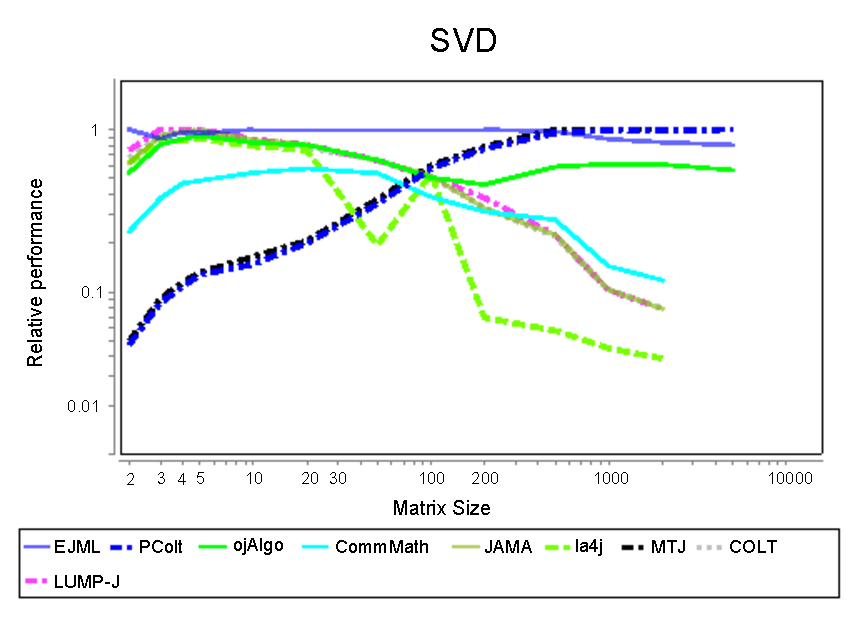
\includegraphics[width=10cm]{figures/svd}
\caption{Graf znázorňující relativní výkon (1 = nejvyšší výkon) různých knihoven při SVD dekompozici. Obrázek je převzat z \cite{svdbench}.}
\label{fig:svd-bench}
\end{center}
\end{figure}

Nejlépe z testu vychází knihovna EJML \cite{svdlib}. Nicméně je nutné poznamenat, že tato knihovna je od stejného autora, jako je daný test. Proto jsem se rozhodl provést vlastní test na reálných datech. Nedělal jsem žádný speciální test, pouze jsem měnil knihovny pro výpočet SVD v rámci již hotového algoritmu. Použil jsem mračno 389002 bodů, nastavil velikost okolí 100 bodů\footnote{To odpovídá průměrně 100 bodům v okolí, tedy i matici 3x100 při výpočtu SVD.} a měřil jsem čas, který výpočet SVD zabere. Měření je uvedeno v tabulce \ref{table:svdlib}.

\begin{table}[ht]
\resizebox{\textwidth}{!} {
\begin{tabular}{|r|r|r|r|r|r|r|r|}
\hline
\textbf{Měření} & \textbf{EJML*} & \textbf{EJML} & \textbf{Jama*} & \textbf{UJMP} & \textbf{CommMath} & \textbf{Colt} & \textbf{jBlas} \\ \hline
\textbf{1} & 88958 & 136998 & 152786 & 157150 & 185178 & 206535 & $>$300000 \\ \hline
\textbf{2} & 88860 & 135831 & 151418 & 156057 & 182576 & 201198 & - \\ \hline
\textbf{Ø} & 88909 & 136415 & 152102 & 156604 & 183877 & 203867 & $>$300000 \\ \hline
\end{tabular}
}
\caption{Tabulka znázorňující časy výpočtu SVD různých knihoven. Časy jsou uvedeny v ms. Knihovny označené * jsou nastavené tak, aby při SVD počítaly pouze matici $V^T$.} 
\label{table:svdlib}
\end{table}

Jak je z tabulky patrné, nejrychlejší je knihovna EJML, stejně jako ve výše uvedeném testování. Rozdíl byl natolik výrazný, že jsem provedl pouze dvě měření, přišlo mi zbytečné měření opakovat na jiných datech. Navíc EJML umožňuje při SVD vypočítávat pouze matici $V^T$, která je pro proložení roviny potřebná, což výrazně zvyšuje celkový výkon. Z těchto důvodů jsem se rozhodl pro výpočty SVD využít EJML.

Dříve v této kapitole jsem odůvodňoval, proč je průměrná velikost okolí zadávána uživatelem. Jedním z argumentů bylo, že uživatel si částečně může zvolit, jestli chce segmentaci provést rychle nebo spíše pomaleji a kvalitněji. Je potřeba zmínit, že rychlost algoritmu není daná pouze vybíráním okolí z kd-stromu. Další velkou složkou z celkového času je právě výpočet SVD při prokládání roviny. Ve skutečnosti prokládání bodů rovinou zabere větší část z celkového času běhu algoritmu, než vybírání bodů z kd-stromu. Nicméně obě tyto hodnoty jsou řádově stejné a dohromady tvoří naprostou většinu z celkové doby běhu. Stejně jako u kd-stromu je i prokládání bodů rovinou je výrazně závislé na počtu vstupních bodů. Mělo by tedy být jasné, že velikost okolí naprosto zásadně ovlivňuje dobu běhu celého algoritmu, uživatel může tedy vhodnou volbou okolí výrazně přizpůsobit celkový čas algoritmu svým potřebám.

Zpět k implementaci algoritmu: jsme ve fázi, kdy máme vybrané okolí bodu a tímto okolím jsme proložili rovinu. Je nutné zmínit, že při prokládání roviny může nastat výjimka, kdy bod nemá žádný bod ve svém okolí nebo má jenom jeden. V takovém případě není proložení roviny možné. Pro takovýto bod tedy nemůžeme vypočítat parametry a je nutné ho zahodit. Nicméně takových bodů by mělo být naprosté minimum a vzhledem k tomu, že bod nema okolí, tak velmi pravděpodobně neleží na žádné rovině a jde spíš o nějakou chybu ve vstupních datech. 

Pokud se rovinu podaří proložit, pokračujeme úpravou této roviny pomocí převažování. Nejprve pro každý bod spočítáme váhu, což je inverze ke vzdálenosti bodu od roviny. Po vypočítání všech vah proložíme znovu rovinu všemi body, nicméně tentokrát využijeme váhy a váženou metody nejmenších čtverců. Implementace vážené varianty metody nejmenších čtverců je téměř stejná jako běžné varianty, jenom se uvažují váhy při výpočtu centroidu a při konstrukce matice, nad kterou se poté provádí SVD. Po proložení roviny se rozhoduje, zda se opět vypočítají váhy a rovina se znovu proloží nebo zda se cyklus ukončí. Ukončení cyklu nastává ve dvou případech, pokud jsme již v desáté iteraci nebo pokud se parametry nové roviny výrazně neliší od poslední iterace.

Ačkoliv tento proces převažování vypadá na první pohled jednoduše, narazil jsem při něm na dva problémy. Prvním je výpočet vah, které se v rámci iterací mění pomalu a provádí se zbytečně velký počet iterací. Jako řešení se nabízí použít inverzi k druhé mocnině vzdálenosti bodu od roviny. Toto řešení funguje poměrně dobře a výrazně snižuje potřebný počet iterací a tím i celkový čas běhu algoritmu. Nicméně i toto řešení má jeden problém, váhy bodů blízko rovině mohou narůstat do výrazně velkých čísel, což může ovlivnit výsledek. Problém nastává také v okamžiku, kdy bod leží přímo na dané ploše. V tu chvíli jeho váha odpovídá hodnotě $\frac{1}{0}$, což Java převede na hodnotu $Double.INFINITY$. Pokud se takováto váha dostane do výpočtu SVD, tak sice nevznikne žádná výjimka a výpočet proběhne, nicméně výsledek je výpočtu je vždy chybný. Tento problém jsme se snažil vyřešit tím, že jsem hodnotu nekonečna nahrazoval nějakou velkou konstantou (zkoušel jsem různé varianty od 10e5 do 10e50), nicméně v tomto případě se výpočet SVD choval velmi nepředvídatelně a vracel špatné výsledky. Takže jediné řešení, které se mi podařilo najít a funguje, je body s \uv{nekonečnou váhou} do výpočtu roviny vůbec nezahrnovat. Toto řešení také není příliš dobré, protože body, které by měly rovinu určovat nejlépe jsme museli z výpočtu vynechat. Naštěstí takovýchto bodů je při výpočtu zanedbatelné množství (v průměru je ovlivněna váha jednoho bodu u 1 - 2\% výpočtů rovin), takže na výslednou segmentaci nemá tento problém žádné rozpoznatelné důsledky.
 

Druhým problémem je otázka, jak správně nastavit hranici, kdy se v rámci dvou iterací roviny už výrazně neliší a proces je ukončen. 


váha = nekonečno


\subsection{Klastrování bodů v akumulátorovém poli}


\subsection{Struktura zdrojového kódu}

Tady bych jen tak nastínil hlavní části toho zdrojáku ve vztahu k tomu předchozímu popisu\ldots

%*****************************************************************************
\chapter{Testování}
\label{chap:test}

\begin{itemize}
 \item Způsob, průběh a výsledky testování.
 \item Srovnání s existujícími řešeními, pokud jsou známy.
\end{itemize} 


%*****************************************************************************
\chapter{Závěr}

\begin{itemize}
\item Zhodnocení splnění cílů DP/BP a  vlastního přínosu práce (při formulaci je třeba vzít v potaz zadání práce).
\item Diskuse dalšího možného pokračování práce.
\end{itemize} 

%*****************************************************************************
% Seznam literatury je v samostatnem souboru reference.bib. Ten
% upravte dle vlastnich potreb, potom zpracujte (a do textu
% zapracujte) pomoci prikazu bibtex a nasledne pdflatex (nebo
% latex). Druhy z nich alespon 2x, aby se poresily odkazy.

% originally following specification for bibliography formating was used
%\bibliographystyle{abbrv}

% Here is an improvment by Petr Dlouhy (April 2010).
% It is mainly for supervisors who expect Czech fomrating rules for references
% Additional feature is live url addresses to sources from your pdf file
% It requires the file csplainnat.bst (included in this sample zipfile).

\bibliographystyle{csplainnat}

%bibliographystyle{plain}
%\bibliographystyle{psc}
%{
%JZ: 11.12.2008 Kdo chce mit v techto ukazkovych odkazech take odkaz na CSTeX:
\def\CS{$\cal C\kern-0.1667em\lower.5ex\hbox{$\cal S$}\kern-0.075em $}
\bibliography{reference}
%}

% M. Dušek radi:
%\bibliographystyle{alpha}
% kdy citace ma tvar [AutorRok] (napriklad [Cook97]). Sice to asi neni podle ceske normy (BTW BibTeX stejne
% neodpovida ceske norme), ale je to nejprehlednejsi.
% 3.5.2009 JZ polemizuje: BibTeX neobvinujte, napiste a poskytnete nam styl (.bst) splnujici citacni normu
% CSN/ISO.

%*****************************************************************************
%*****************************************************************************
\appendix



%*****************************************************************************
\chapter{Pokyny a návody k formátování textu práce}
\textbf{\large Tato příloha samozřejmě nebude součástí vaší práce. Slouží pouze jako příklad formátování textu.}

Používat se dají všechny příkazy systému \LaTeX. Existuje velké množství volně přístupné dokumentace,
tutoriálů, příruček a dalších materiálů v elektronické podobě. Výchozím bodem, kromě Googlu, může být stránka
CSTUG (Czech Tech Users Group) \cite{CSTUG}. Tam najdete odkazy na další materiály.  Vetšinou dostačující a
přehledně organizovanou elektronikou dokumentaci najdete například na \cite{latexdocweb} nebo \cite{latexwiki}.

Existují i různé nadstavby nad systémy \TeX{} a \LaTeX, které výrazně usnadní psaní textu zejména
začátečníkům. Velmi rozšířený v Linuxovém prostředí je systém Kile.


\section{Vkládání obrázků}
Obrázky se umísťují do plovoucího prostředí \verb|figure|. Každý obrázek by měl obsahovat \textbf{název}
(\verb|\caption|) a \textbf{návěští} (\verb|\label|). Použití příkazu pro vložení obrázku
\\\verb|\includegraphics| je podmíněno aktivací (načtením) balíku graphicx příkazem\\
\verb|\usepackage{graphicx}|.

Budete-li zdrojový text zpracovávat pomocí programu \verb|pdflatex|, očekávají se obrázky s příponou
\verb|*.pdf|\footnote{pdflatex umí také formáty PNG a JPG.}, použijete-li k formátování \verb|latex|,
očekávají se obrázky s příponou \verb|*.eps|.\footnote{Vzájemnou konverzi mezi snad všemi typy obrazku včetně
změn vekostí a dalších vymožeností vám může zajistit balík ImageMagic 
(http://www.imagemagick.org/script/index.php). Je dostupný pod Linuxem, Mac OS i MS Windows. Důležité jsou
zejména příkazy convert a identify.}

\begin{figure}[ht]
\begin{center}

\includegraphics[width=5cm]{figures/LogoCVUT}
\caption{Popiska obrázku}
\label{fig:logo}
\end{center}
\end{figure}

Příklad vložení obrázku:
\begin{verbatim}
\begin{figure}[h]
\begin{center}

\includegraphics[width=5cm]{figures/LogoCVUT}
\caption{Popiska obrazku}
\label{fig:logo}
\end{center}
\end{figure}
\end{verbatim}

\section{Kreslení obrázků}
Zřejmě každý z vás má nějaký oblíbený nástroj pro tvorbu obrázků. Jde jen o to, abyste dokázali obrázek uložit
v požadovaném formátu nebo jej do něj konvertovat (viz předchozí kapitola). Je zřejmě vhodné kreslit obrázky
vektorově. Celkem oblíbený, na ovládání celkem jednoduchý a přitom dostatečně mocný je například program Inkscape.

Zde stojí za to upozornit na kreslící programe Ipe \cite{ipe}, který dokáže do obrázku vkládat komentáře přímo
v latexovském formátu (vzroce, stejné fonty atd.). Podobné věci umí na Linuxové platformě nástroj Xfig.

Za pozornost ještě stojí schopnost editoru Ipe importovat obrázek (jpg nebo bitmap) a krelit do něj latexovské
popisky a komentáře. Výsledek pak umí exportovat přímo do pdf.

\section{Tabulky}
Existuje více způsobů, jak sázet tabulky. Například je možno použít prostředí \verb|table|, které je velmi
podobné prostředí \verb|figure|.

\begin{table}
\begin{center}
\begin{tabular}{|c|l|l|}
\hline
\textbf{DTD} & \textbf{construction} & \textbf{elimination} \\
\hline
$\mid$ & \verb+in1|A|B a:sum A B+ & \verb+case([_:A]a)([_:B]a)ab:A+\\
&\verb+in1|A|B b:sum A B+ & \verb+case([_:A]b)([_:B]b)ba:B+\\
\hline
$+$&\verb+do_reg:A -> reg A+&\verb+undo_reg:reg A -> A+\\
\hline
$*,?$& the same like $\mid$ and $+$ & the same like $\mid$ and $+$\\
& with \verb+emtpy_el:empty+ & with \verb+emtpy_el:empty+\\
\hline
R(a,b) & \verb+make_R:A->B->R+ & \verb+a: R -> A+\\
 & & \verb+b: R -> B+\\
\hline
\end{tabular}
\end{center}
\caption{Ukázka tabulky}
\label{tab:tab1}
\end{table}

Zdrojový text tabulky \ref{tab:tab1} vypadá takto:
\begin{verbatim}
\begin{table}
\begin{center}
\begin{tabular}{|c|l|l|}
\hline
\textbf{DTD} & \textbf{construction} & \textbf{elimination} \\
\hline
$\mid$ & \verb+in1|A|B a:sum A B+ & \verb+case([_:A]a)([_:B]a)ab:A+\\
&\verb+in1|A|B b:sum A B+ & \verb+case([_:A]b)([_:B]b)ba:B+\\
\hline
$+$&\verb+do_reg:A -> reg A+&\verb+undo_reg:reg A -> A+\\
\hline
$*,?$& the same like $\mid$ and $+$ & the same like $\mid$ and $+$\\
& with \verb+emtpy_el:empty+ & with \verb+emtpy_el:empty+\\
\hline
R(a,b) & \verb+make_R:A->B->R+ & \verb+a: R -> A+\\
 & & \verb+b: R -> B+\\
\hline
\end{tabular}
\end{center}
\caption{Ukázka tabulky}
\label{tab:tab1}
\end{table}
\begin{table}
\end{verbatim}

\section{Odkazy v textu}
\subsection{Odkazy na literaturu}
Jsou realizovány příkazem \verb|\cite{odkaz}|. 

Seznam literatury je dobré zapsat do samostatného souboru a ten pak zpracovat programem bibtex (viz soubor
\verb|reference.bib|). Zdrojový soubor pro \verb|bibtex| vypadá například takto:
\begin{verbatim}
@Article{Chen01,
  author  = "Yong-Sheng Chen and Yi-Ping Hung and Chiou-Shann Fuh",
  title   = "Fast Block Matching Algorithm Based on 
             the Winner-Update Strategy",
  journal = "IEEE Transactions On Image Processing",
  pages   = "1212--1222",
  volume  =  10,
  number  =   8,
  year    = 2001,
}

@Misc{latexdocweb,
  author  = "",
  title   = "{\LaTeX} --- online manuál",
  note    = "\verb|http://www.cstug.cz/latex/lm/frames.html|",
  year    = "",
}
...
\end{verbatim}

%11.12.2008, 3.5.2009
\textbf{Pozor:} Sazba názvů odkazů je dána Bib\TeX{} stylem\\ (\verb|\bibliographystyle{abbrv}|). 
%Budete-li používat české prostředí (\verb|\usepackage[czech]{babel}|), 
Bib\TeX{} tedy obvykle vysází velké pouze počáteční písmeno z názvu zdroje, 
ostatní písmena zůstanou malá bez ohledu na to, jak je napíšete. 
Přesněji řečeno, styl může zvolit pro každý typ publikace jiné konverze. 
Pro časopisecké články třeba výše uvedené, jiné pro monografie (u nich často bývá 
naopak velikost písmen zachována).

Pokud chcete Bib\TeX u napovědět, která písmena nechat bez konverzí 
(viz \texttt{title = "\{$\backslash$LaTeX\} -{}-{}- online manuál"} 
v~předchozím příkladu), je nutné příslušné písmeno (zde celé makro) uzavřít 
do složených závorek. Pro přehlednost je proto vhodné celé parametry 
uzavírat do uvozovek (\texttt{author = "\dots"}), nikoliv do složených závorek.

Odkazy na literaturu ve zdrojovém textu se pak zapisují:
\begin{verbatim}
Podívejte se na \cite{Chen01}, 
další detaily najdete na \cite{latexdocweb}
\end{verbatim}

Vazbu mezi soubory \verb|*.tex| a \verb|*.bib| zajistíte příkazem 
\verb|\bibliography{}| v souboru \verb|*.tex|.  V našem případě tedy zdrojový 
dokument \verb|thesis.tex| obsahuje příkaz\\
\verb|\bibliography{reference}|.

Zpracování zdrojového textu s odkazy se provede postupným voláním programů\\
\verb|pdflatex <soubor>| (případně \verb|latex <soubor>|), \verb|bibtex <soubor>| 
a opět\\ \verb|pdflatex <soubor>|.\footnote{První volání \texttt{pdflatex} 
vytvoří soubor s~koncovkou \texttt{*.aux}, který je vstupem pro program 
\texttt{bibtex}, pak je potřeba znovu zavolat program \texttt{pdflatex} 
(\texttt{latex}), který tentokrát zpracuje soubory s příponami \texttt{.aux} a 
\texttt{.tex}. 
Informaci o případných nevyřešených odkazech (cross-reference) vidíte přímo při 
zpracovávání zdrojového souboru příkazem \texttt{pdflatex}. Program \texttt{pdflatex} 
(\texttt{latex}) lze volat vícekrát, pokud stále vidíte nevyřešené závislosti.}


Níže uvedený příklad je převzat z dříve existujících pokynů studentům, kteří 
dělají svou diplomovou nebo bakalářskou práci v~Grafické skupině.\footnote{Několikrát 
jsem byl upozorněn, že web s těmito pokyny byl zrušen, proto jej zde přímo necituji. 
Nicméně příklad sám o sobě dokumentuje obecně přijímaný konsensus ohledně citací 
v~bakalářských a diplomových pracích na KP.} Zde se praví:
\begin{small}
\begin{verbatim}
...
j) Seznam literatury a dalších použitých pramenů, odkazy na WWW stránky, ...
 Pozor na to, že na veškeré uvedené prameny se musíte v textu práce 
 odkazovat -- [1]. 
Pramen, na který neodkazujete, vypadá, že jste ho vlastně nepotřebovali 
a je uveden jen do počtu. Příklad citace knihy [1], článku v časopise [2], 
stati ve sborníku [3] a html odkazu [4]: 
[1] J. Žára, B. Beneš;, and P. Felkel. 
     Moderní počítačová grafika. Computer Press s.r.o, Brno, 1 edition, 1998. 
     (in Czech). 
[2] P. Slavík. Grammars and Rewriting Systems as Models for Graphical User 
     Interfaces. Cognitive Systems, 4(4--3):381--399, 1997. 
[3] M. Haindl, Š. Kment, and P. Slavík. Virtual Information Systems. 
     In WSCG'2000 -- Short communication papers, pages 22--27, Pilsen, 2000. 
     University of West Bohemia. 
[4] Knihovna grafické skupiny katedry počítačů: 
     http://www.cgg.cvut.cz/Bib/library/ 
\end{verbatim}
\end{small}
\ldots{} abychom výše citované odkazy skutečně našli v (automaticky generovaném) seznamu literatury tohoto
textu, musíme je nyní alespoň jednou citovat: Kniha \cite{kniha}, článek v~časopisu \cite{clanek}, příspěvek
na konferenci \cite{sbornik}, www odkaz \cite{www}.

Ještě přidáme další ukázku citací online zdrojů podle české normy. Odkaz na wiki o frameworcich
\cite{wiki:framework} a ORM \cite{wiki:orm}. Použití viz soubor \verb|reference.bib|. V seznamu literatury by
nyní měly být živé odkazy na zdroje. V \verb|reference.bib| je zcela nový typ publikace. Detaily dohledal a
dodal Petr Dlouhý v dubnu 2010. Podrobnosti najdete ve zdrojovém souboru tohoto textu v komentáři u příkazu
\verb|\thebibliography|.

\subsection{Odkazy na obrázky, tabulky a kapitoly}
\begin{itemize}
\item Označení místa v textu, na které chcete později čtenáře práce odkázat, se provede příkazem
\verb|\label{navesti}|. Lze použít v prostředích \verb|figure| a  \verb|table|, ale též za názvem kapitoly
nebo podkapitoly.
\item Na návěští se odkážeme příkazem \verb|\ref{navesti}| nebo \verb|\pageref{navesti}|.
\end{itemize}

\section{Rovnice, centrovaná, číslovaná matematika}
Jednoduchý matematický výraz zapsaný přímo do textu se vysází pomocí prostředí \verb|math|, resp. zkrácený
zápis pomocí uzavření textu rovnice mezi znaky \verb|$|.

Kód \verb|$ S = \pi * r^2 $| bude vysázen takto: $ S = \pi * r^2 $.

Pokud chcete nečíslované rovnice, ale umístěné centrovaně na samostatné řádky, pak lz  použít prostředí
\verb|displaymath|, resp. zkrácený zápis pomocí uzavření textu rovnice mezi znaky \verb|$$|. Zdrojový kód:
\begin{verb}
|$$ S = \pi * r^2 $$|
\end{verb}
bude pak vysázen takto:
$$ S = \pi * r^2 $$

Chcete-li mít rovnice číslované, je třeba použít prostředí \verb|eqation|. Kód:
\begin{verbatim}
\begin{equation}
  S = \pi * r^2
\end{equation}

\begin{equation}
  V = \pi * r^3
\end{equation}
\end{verbatim}
je potom vysázen takto:
\begin{equation}
  S = \pi * r^2
\end{equation}

\begin{equation}
  V = \pi * r^3
\end{equation}

\section{Kódy programu}
Chceme-li vysázet například část zdrojového kódu programu (bez formátování), hodí se prostředí \verb|verbatim|: 
\begin{verbatim}
         (* nickname2 *)
Lego> Refine in1
             (do_reg (nickname1 h));
Refine by  in1 (do_reg (nickname1 h))
   ?4 : pcdata
   ?5 : pcdata
          (* surname2 *)
Lego> Refine surname1 h;
Refine by  surname1 h
   ?5 : pcdata
          (* email2 *)
Lego> Refine undo_reg (email1 h);
Refine by  undo_reg (email1 h)
*** QED ***
\end{verbatim}

\section{Další poznámky}
\subsection{České uvozovky}
V souboru \verb|k336_thesis_macros.tex| je příkaz \verb|\uv{}| pro sázení českých uvozovek. \uv{Text uzavřený
do českých uvozovek.}

% JZ: 3.5.2009 \chapter z book zajistí automaticky
%\subsection{Začátky kapitol na liché stránky}
%Ve výsledném textu je dobré, když každá kapitola začíná na liché stránce. Tedy použijte:
%\begin{verbatim}
%  \cleardoublepage\include{1_uvod}
%  \cleardoublepage\include{2_teorie}
%   atd.\ldots{}
%\end{verbatim}

%*****************************************************************************
\chapter{Seznam použitých zkratek}

\begin{description}
\item[2D] Two-Dimensional
\item[ABN] Abstract Boolean Networks
\item[ASIC] Application-Specific Integrated Circuit
\end{description}
\vdots


%*****************************************************************************
\chapter{Instalační a uživatelská příručka}
Tato příloha velmi žádoucí zejména u softwarových implementačních prací


%*****************************************************************************
\chapter{Obsah přiloženého CD}
\label{chap:CD}
Tato příloha je povinná pro každou práci. Každá práce musí totiž obsahovat přiložené CD. Viz dále.

Může vypadat například takto. Váš seznam samozřejmě bude odpovídat typu vaší práce. (viz \cite{infodp}):

%\begin{figure}[h]
%\begin{center}
%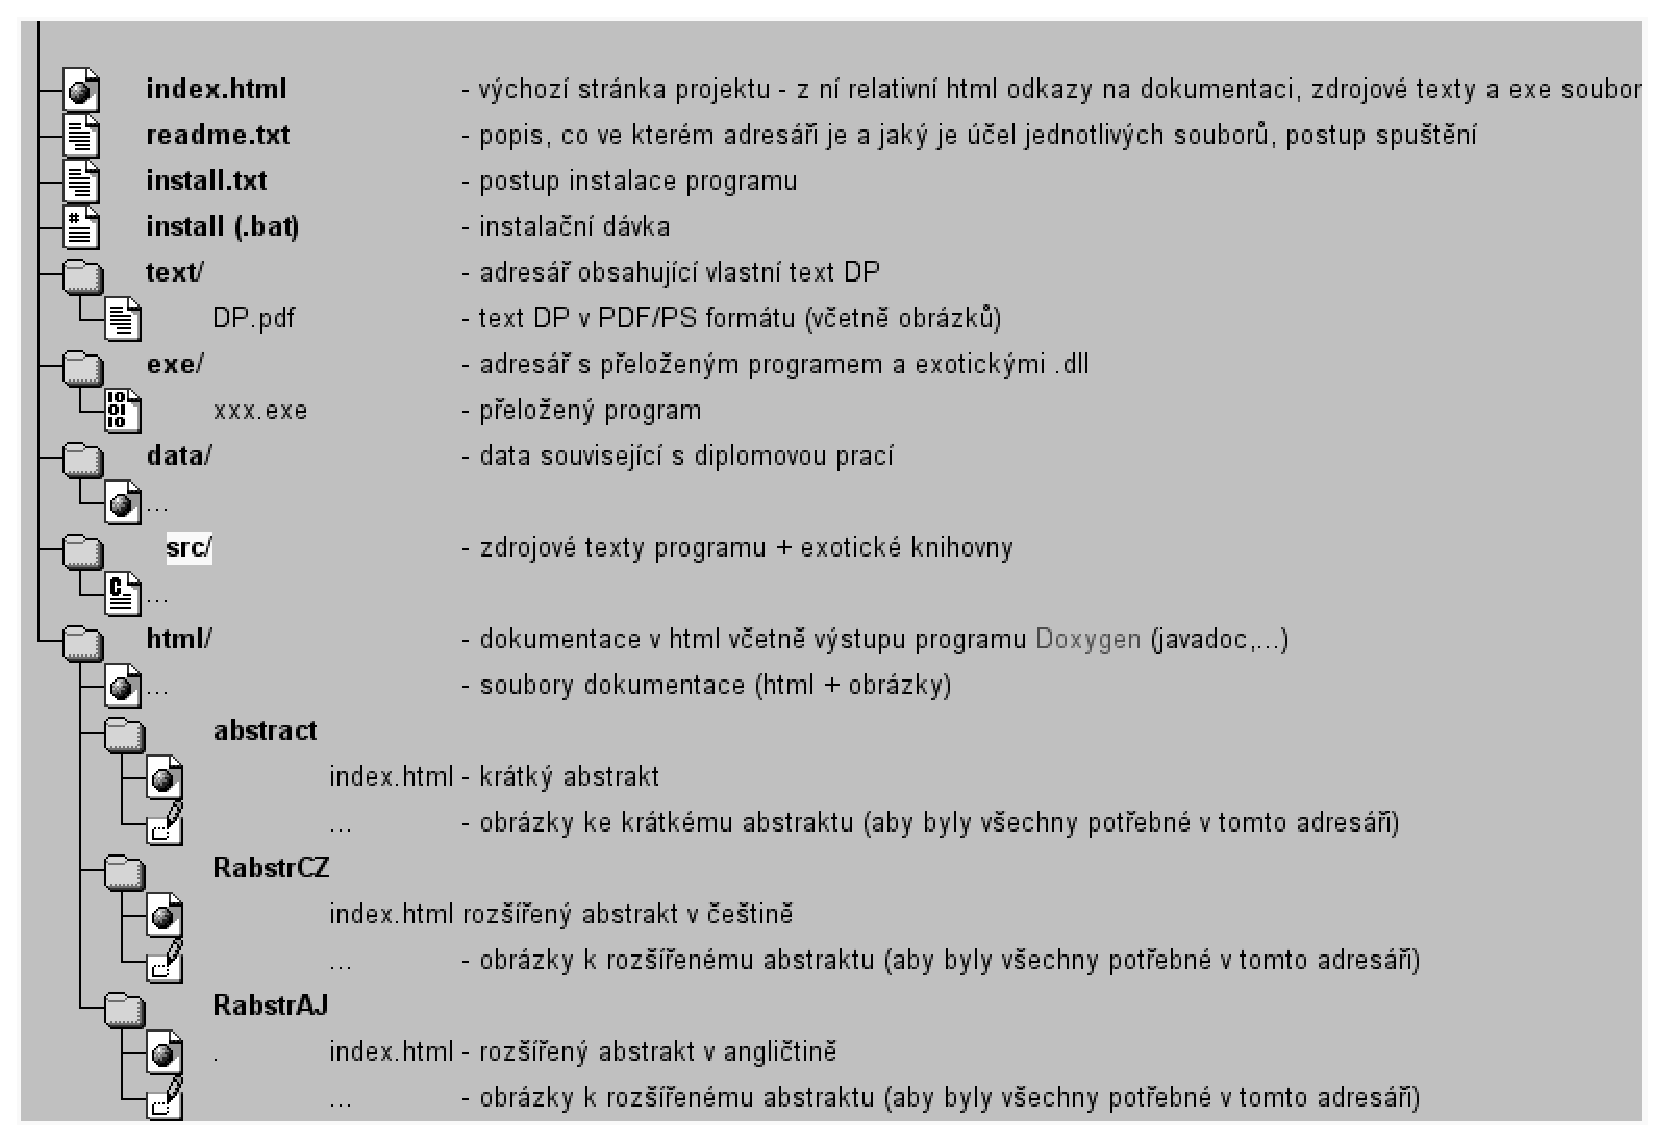
\includegraphics[width=14cm]{figures/seznamcd}
%\caption{Seznam přiloženého CD --- příklad}
%\label{fig:seznamcd}
%\end{center}
%\end{figure}

Na GNU/Linuxu si strukturu přiloženého CD můžete snadno vyrobit příkazem:\\ 
\verb|$ tree . >tree.txt|\\
Ve vzniklém souboru pak stačí pouze doplnit komentáře.

Z \textbf{README.TXT} (případne index.html apod.)  musí být rovněž zřejmé, jak programy instalovat, spouštět a
jaké požadavky mají tyto programy na hardware.

Adresář \textbf{text}  musí obsahovat soubor s vlastním textem práce v PDF nebo PS formátu, který bude později
použit pro prezentaci diplomové práce na WWW.

\end{document}
